
\chapter{Extended Atari Benchmark (Experiment 3)}
\label{chap:exp3}

In this chapter I extend the Atari benchmark of Chapter~\ref{chap:exp2} in two ways: the training budget grows from 5M to 20M environment steps per seed, and a third environment (Seaquest) is added to widen the task distribution. The primary finding is that the two aggregation lenses disagree --- the interquartile mean (IQM) says DQN wins the cross-environment aggregate (0.443 vs 0.277), while the pairwise probability of improvement says PPO wins ($P(\text{DQN}>\text{PPO})=0.393$). Beneath both aggregates the per-environment picture is split: DQN dominates Breakout by a factor of 3.5, while PPO wins Pong (1.8$\times$) and Seaquest (1.6$\times$). A secondary finding is that the training pipeline is bitwise deterministic on the target hardware (RTX~4090), allowing retrained seeds to be compared against the originals as a reproducibility check. All evaluation metrics are defined in Section~\ref{sec:eval-framework}.

%% ------------------------------------------------------------------
\section{Motivation}
\label{sec:exp3-motivation}

Chapter~\ref{chap:exp2} flagged $M=2$ as a fragility point for cross-environment aggregates. When only two environments are pooled, one environment's result dominates any IQM or performance-profile curve, and the aggregate becomes a noisy restatement of whichever environment has the larger dynamic range. Experiment~3 addresses this by adding Seaquest --- an Atari game where both algorithms make visible progress --- bringing the Atari task suite to $M=3$.

The secondary motivation is budget. Chapter~\ref{chap:exp2}'s 5M-step runs sit well below the 50M-frame budgets used in the original DQN and PPO papers. Experiment~3 pushes per-run training to 20M steps (80M frames) to see whether the ranking between DQN and PPO depends on the training budget.

%% ------------------------------------------------------------------
\section{Experimental Setup}
\label{sec:exp3-setup}

Hardware and the CnnPolicy / frame-stack / reward-clipping pipeline are identical to Chapter~\ref{chap:exp2} (see Section~\ref{sec:atari-hardware}). The changes are:

\begin{itemize}
  \item \textbf{Training budget.} 20M timesteps per seed per environment (Experiment~2 used 5M).
  \item \textbf{Environment set.} \texttt{PongNoFrameskip-v4}, \texttt{BreakoutNoFrameskip-v4}, \texttt{SeaquestNoFrameskip-v4} (Experiment~2 used only Pong and Breakout).
  \item \textbf{Seeds.} 10 seeds per algorithm per environment, drawn from master seed 20260301.
  \item \textbf{DQN replay buffer.} \texttt{buffer\_size=100{,}000} with \texttt{optimize\_memory\_usage=True}. The intended buffer size was 400K; the smaller buffer was an oversight during training-script configuration and is discussed in the Limitations section.
  \item \textbf{Evaluation frequency.} 100K steps (200 checkpoints per run), 10 evaluation episodes per checkpoint.
\end{itemize}

%% ------------------------------------------------------------------
\section{Hypotheses}
\label{sec:exp3-hypotheses}

Before running the experiments, I formed the following expectations:

\begin{enumerate}
  \item \textbf{PPO continues to dominate Pong.} Pong is a policy-gradient-friendly task with a dense reward signal. Extending the budget should not change the ranking.
  \item \textbf{DQN continues to edge Breakout.} Breakout rewards value-based exploitation of learned state-action values, and Experiment~2 already showed DQN ahead. More training should let DQN widen the gap.
  \item \textbf{Both algorithms make meaningful progress on Seaquest.} Seaquest was chosen as an environment where both algorithms are known to learn non-trivial policies at Nature-paper budgets.
  \item \textbf{The PPO-dominance aggregate from Experiment~2 should survive.} Experiment~2 found $P(\text{PPO}>\text{DQN})=0.648$; adding Seaquest and extending the budget should not flip the aggregate.
  \item \textbf{Cross-environment aggregates will still be fragile at $M=3$.} A single environment can still dominate the profile if its per-environment IQM is much larger than the others.
\end{enumerate}

%% ------------------------------------------------------------------
\section{Training Summary}
\label{sec:exp3-training}

30 runs total (2 algorithms $\times$ 3 environments $\times$ 10 seeds). Training timing for the original run was lost due to an instrumentation issue; all reported wall-clock figures come from retrained reproducibility runs. Timing is now complete for all 60 seeds (30/30 DQN, 30/30 PPO). Evaluation scores are also complete for all 30 runs.

Wall-clock totals on RTX~4090: DQN $\approx$72.5\,h total (27.7\,h Pong, 17.4\,h Breakout, 27.4\,h Seaquest); PPO $\approx$107.5\,h total (37.0\,h Pong, 33.7\,h Breakout, 36.8\,h Seaquest). See Table~\ref{tab:exp3-timing} for per-seed detail.

%% ------------------------------------------------------------------
\section{Per-Environment Results}
\label{sec:exp3-per-env}

\subsection{Pong}
\label{sec:exp3-pong}

PPO nearly solves Pong at the 20M-step budget, with a mean raw return of 19.78 ($\sigma=2.17$). DQN makes clear progress but shows high per-seed variance, with a mean of 11.20 and the weakest seeds still in negative territory. This matches Hypothesis~H3.1. Figure~\ref{fig:exp3-lc-pong} shows the learning curves.

\begin{figure}[htbp!]
  \centering
  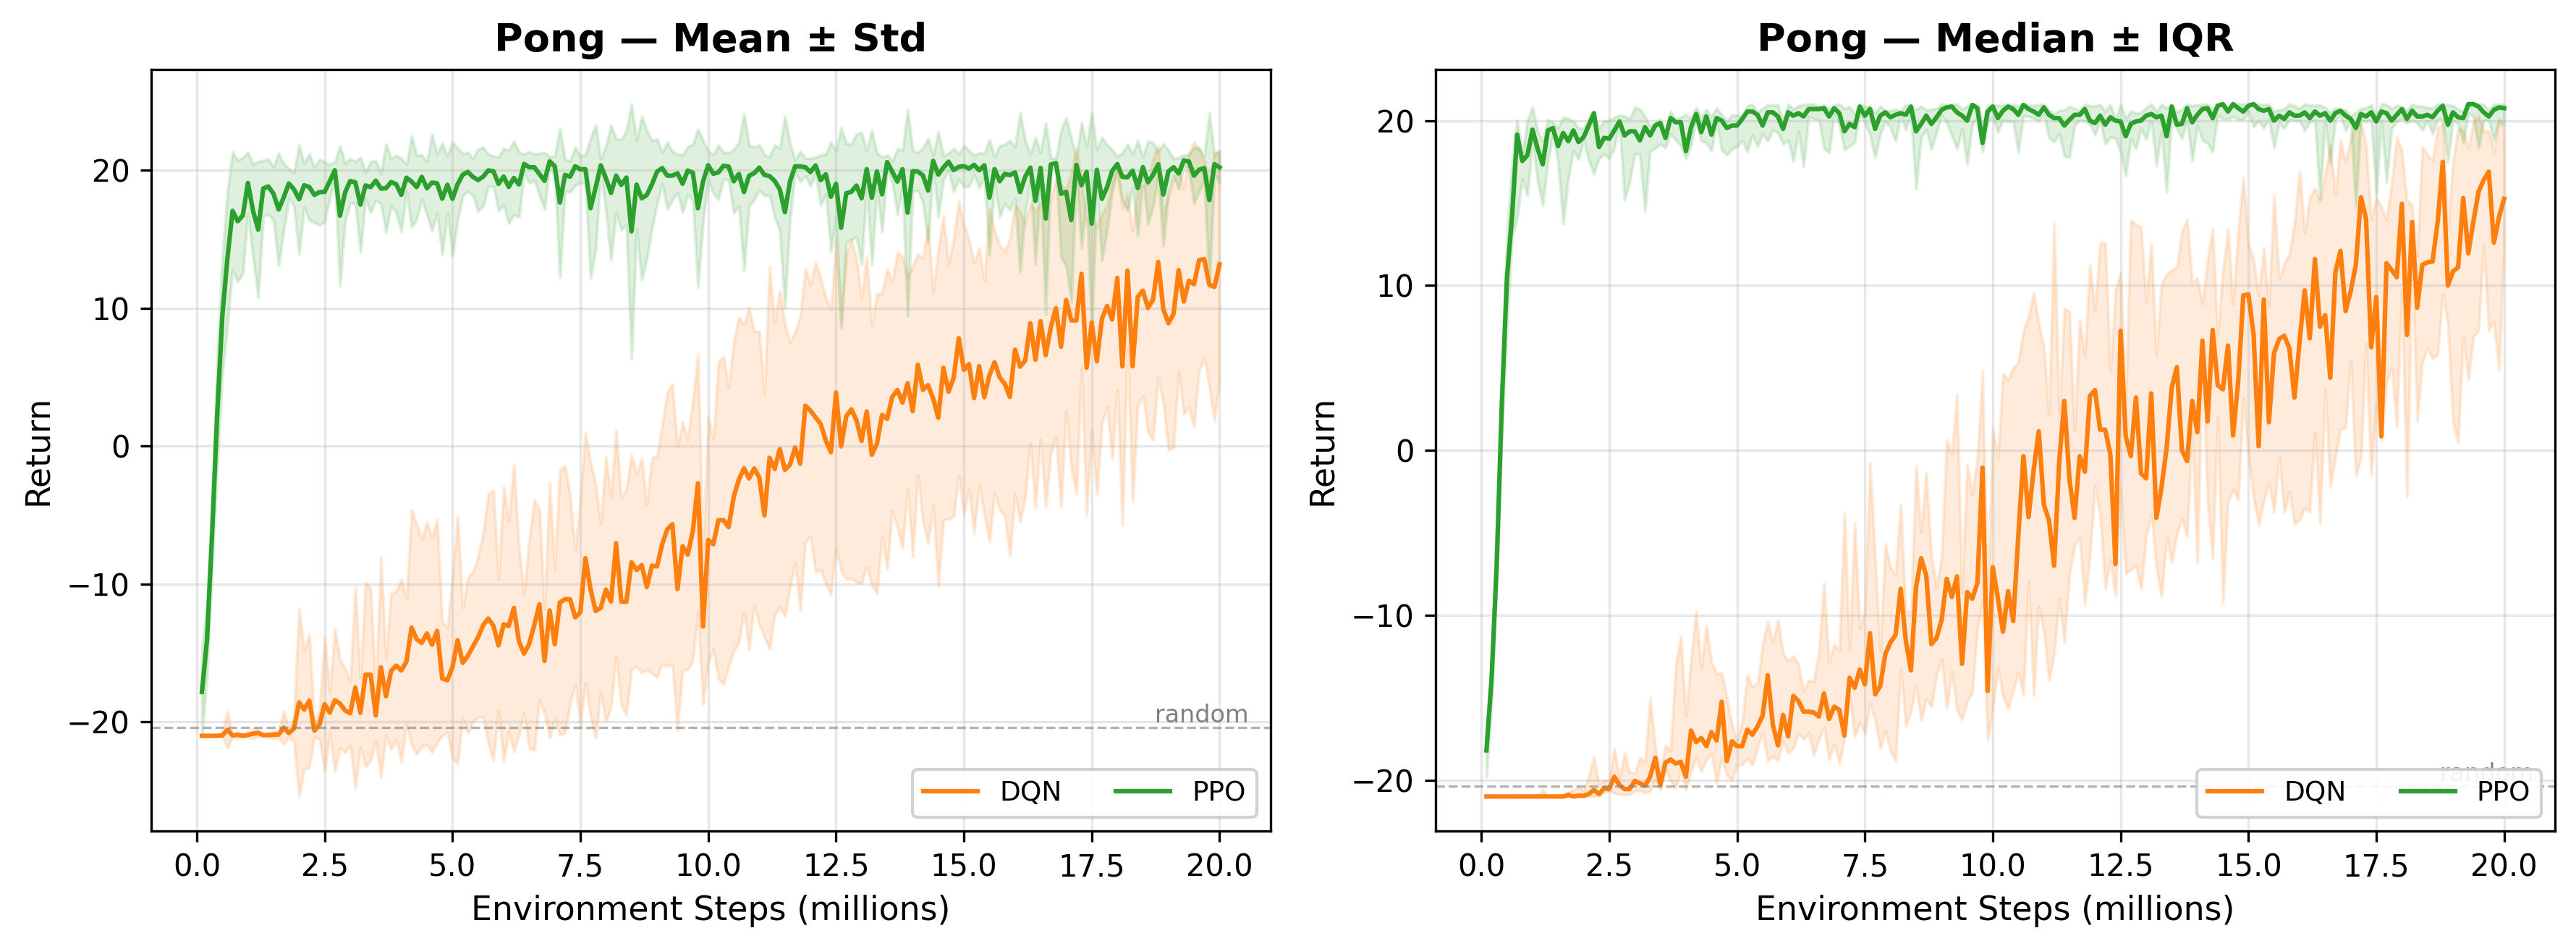
\includegraphics[width=\linewidth]{6_exp3_atari_extended/assets/learning_curves_pong.png}
  \caption[Learning curves on Pong, 20M steps]{Learning curves on Pong, 10 seeds per algorithm, 20M steps. PPO converges near the
           maximum return; DQN shows high per-seed variance.}
  \label{fig:exp3-lc-pong}
\end{figure}

\subsection{Breakout}
\label{sec:exp3-breakout}

DQN dominates Breakout decisively, with a mean return of 229.07 versus PPO's 65.50 --- a $3.5\times$ margin. Per-seed spread is wide (DQN seeds range from roughly 152 to 338) but the gap between the two algorithms is decisive at every seed. This matches Hypothesis~H3.2 and is the largest per-environment margin in the experiment. Figure~\ref{fig:exp3-lc-breakout} shows the learning curves.

\begin{figure}[htbp!]
  \centering
  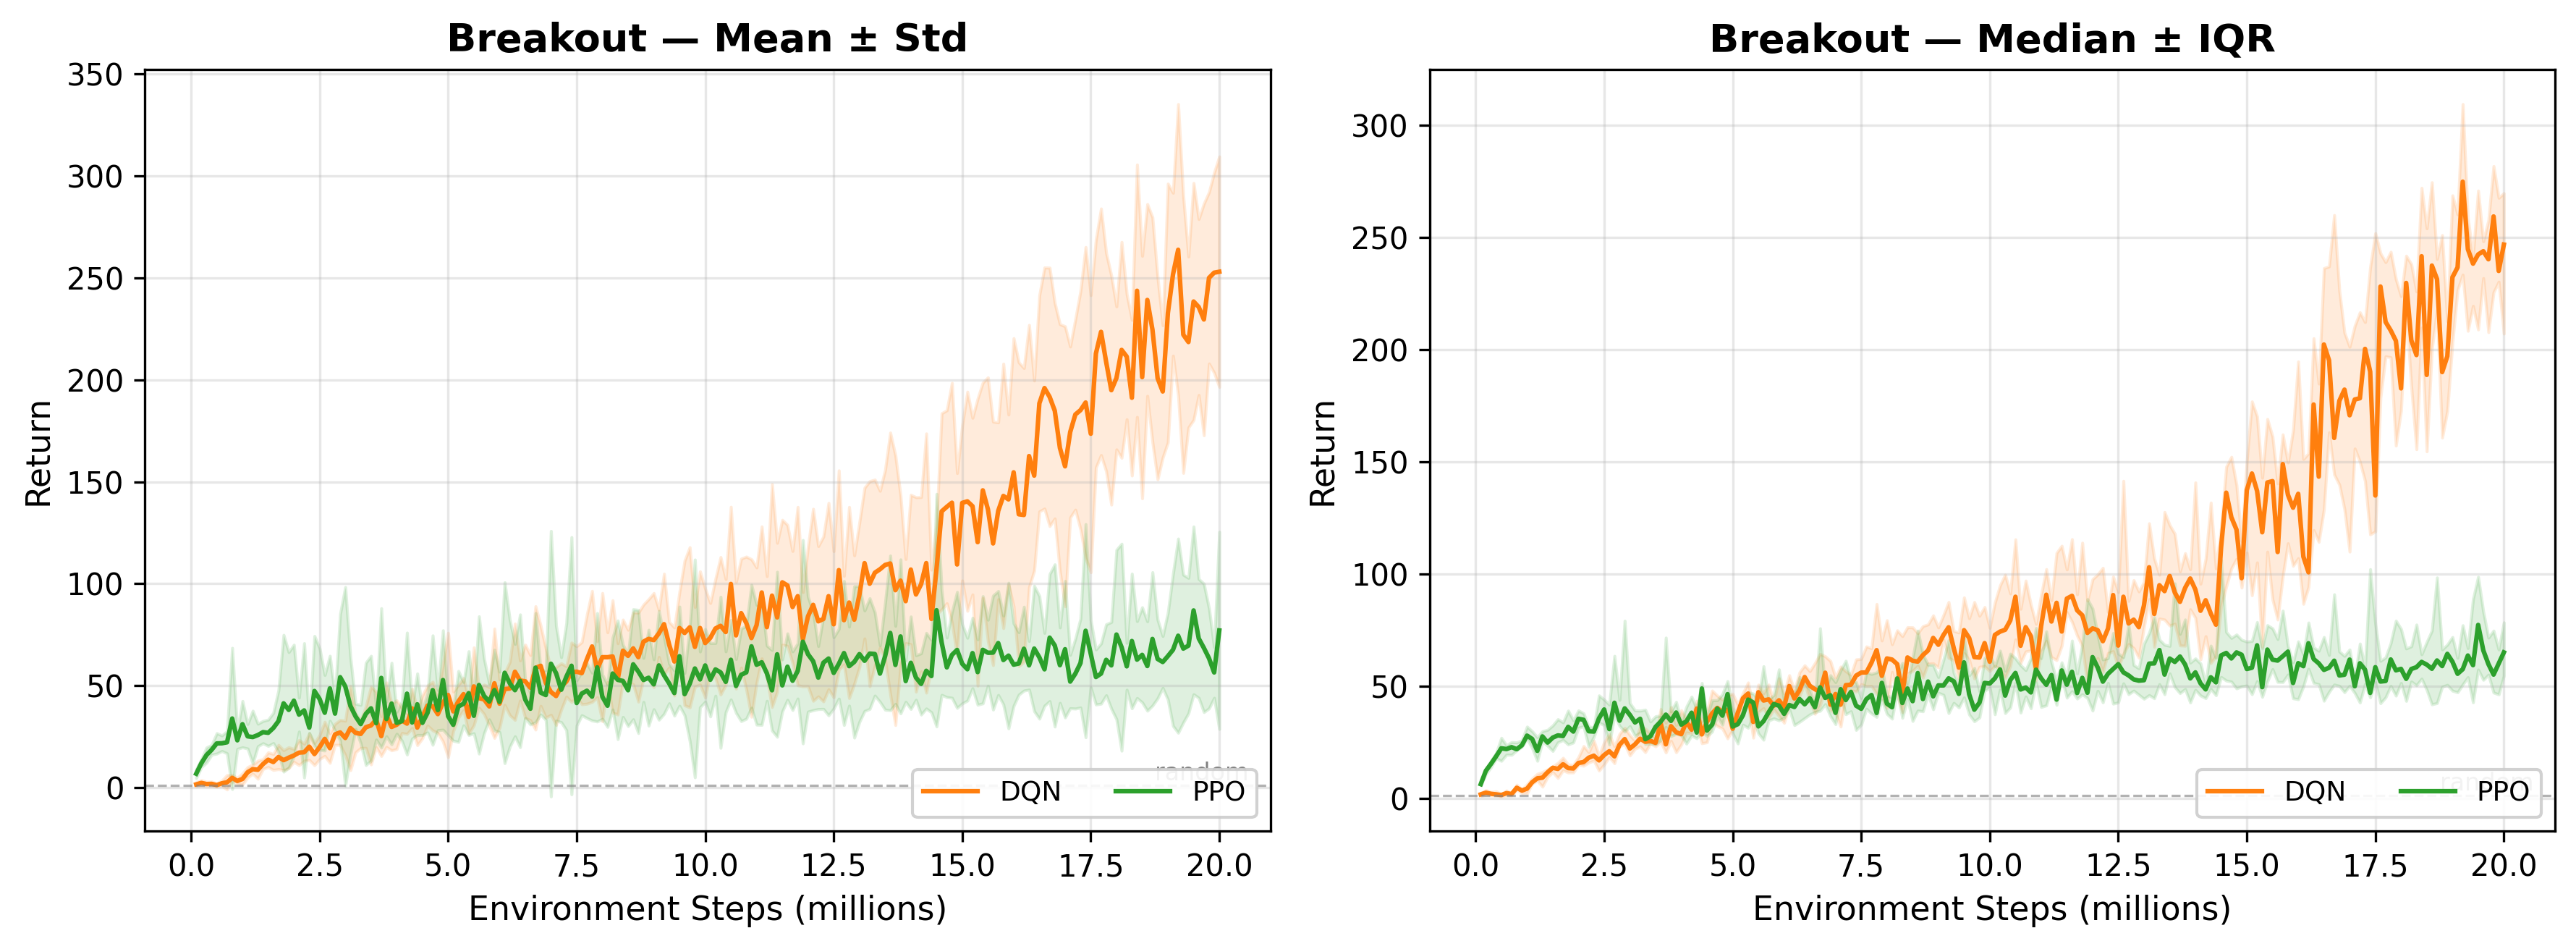
\includegraphics[width=\linewidth]{6_exp3_atari_extended/assets/learning_curves_breakout.png}
  \caption[Learning curves on Breakout, 20M steps]{Learning curves on Breakout, 10 seeds per algorithm, 20M steps. DQN achieves a
           $3.5\times$ mean-return advantage over PPO.}
  \label{fig:exp3-lc-breakout}
\end{figure}

\subsection{Seaquest}
\label{sec:exp3-seaquest}

PPO wins Seaquest with a mean return of 1173.92 versus DQN's 714.00 (a $1.64\times$ advantage). Both algorithms show the hallmark Seaquest plateau --- rapid initial improvement followed by a long period of minor gains --- but PPO's plateau is higher and tighter across seeds. Both algorithms clearly exceed the random baseline ($\approx68$), confirming Hypothesis~H3.3. Figure~\ref{fig:exp3-lc-seaquest} shows the learning curves.

\begin{figure}[htbp!]
  \centering
  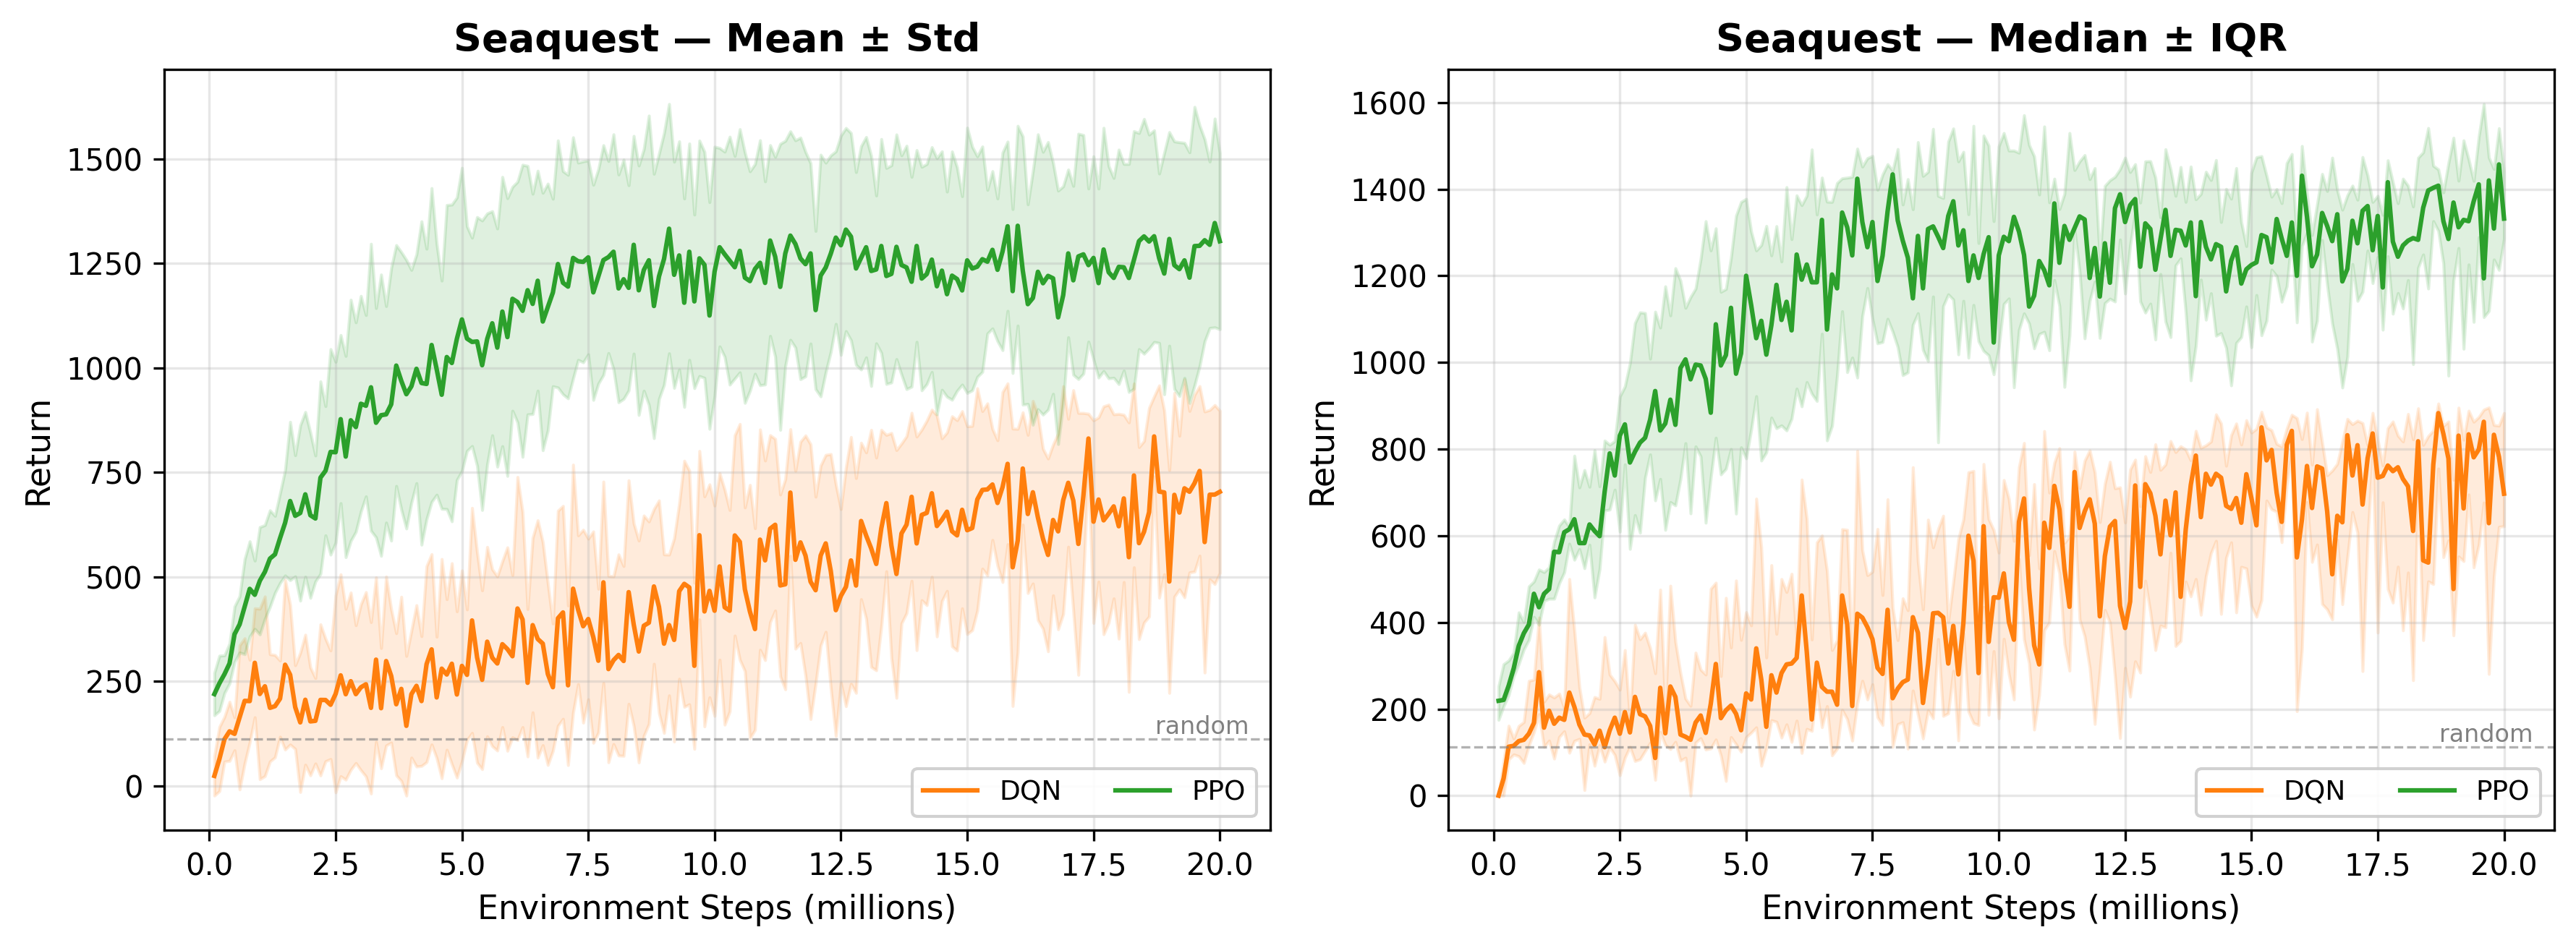
\includegraphics[width=\linewidth]{6_exp3_atari_extended/assets/learning_curves_seaquest.png}
  \caption[Learning curves on Seaquest, 20M steps]{Learning curves on Seaquest, 10 seeds per algorithm, 20M steps. Both algorithms
           plateau after initial rapid improvement; PPO's plateau is higher.}
  \label{fig:exp3-lc-seaquest}
\end{figure}

\subsection{Combined Learning Curves}
\label{sec:exp3-combined-lc}

Figure~\ref{fig:exp3-lc-combined} overlays all three environments on a normalised $y$-axis. The combined view is dominated by whichever environment has the highest normalised ceiling; per-environment curves above are the primary evidence.

\begin{figure}[htbp!]
  \centering
  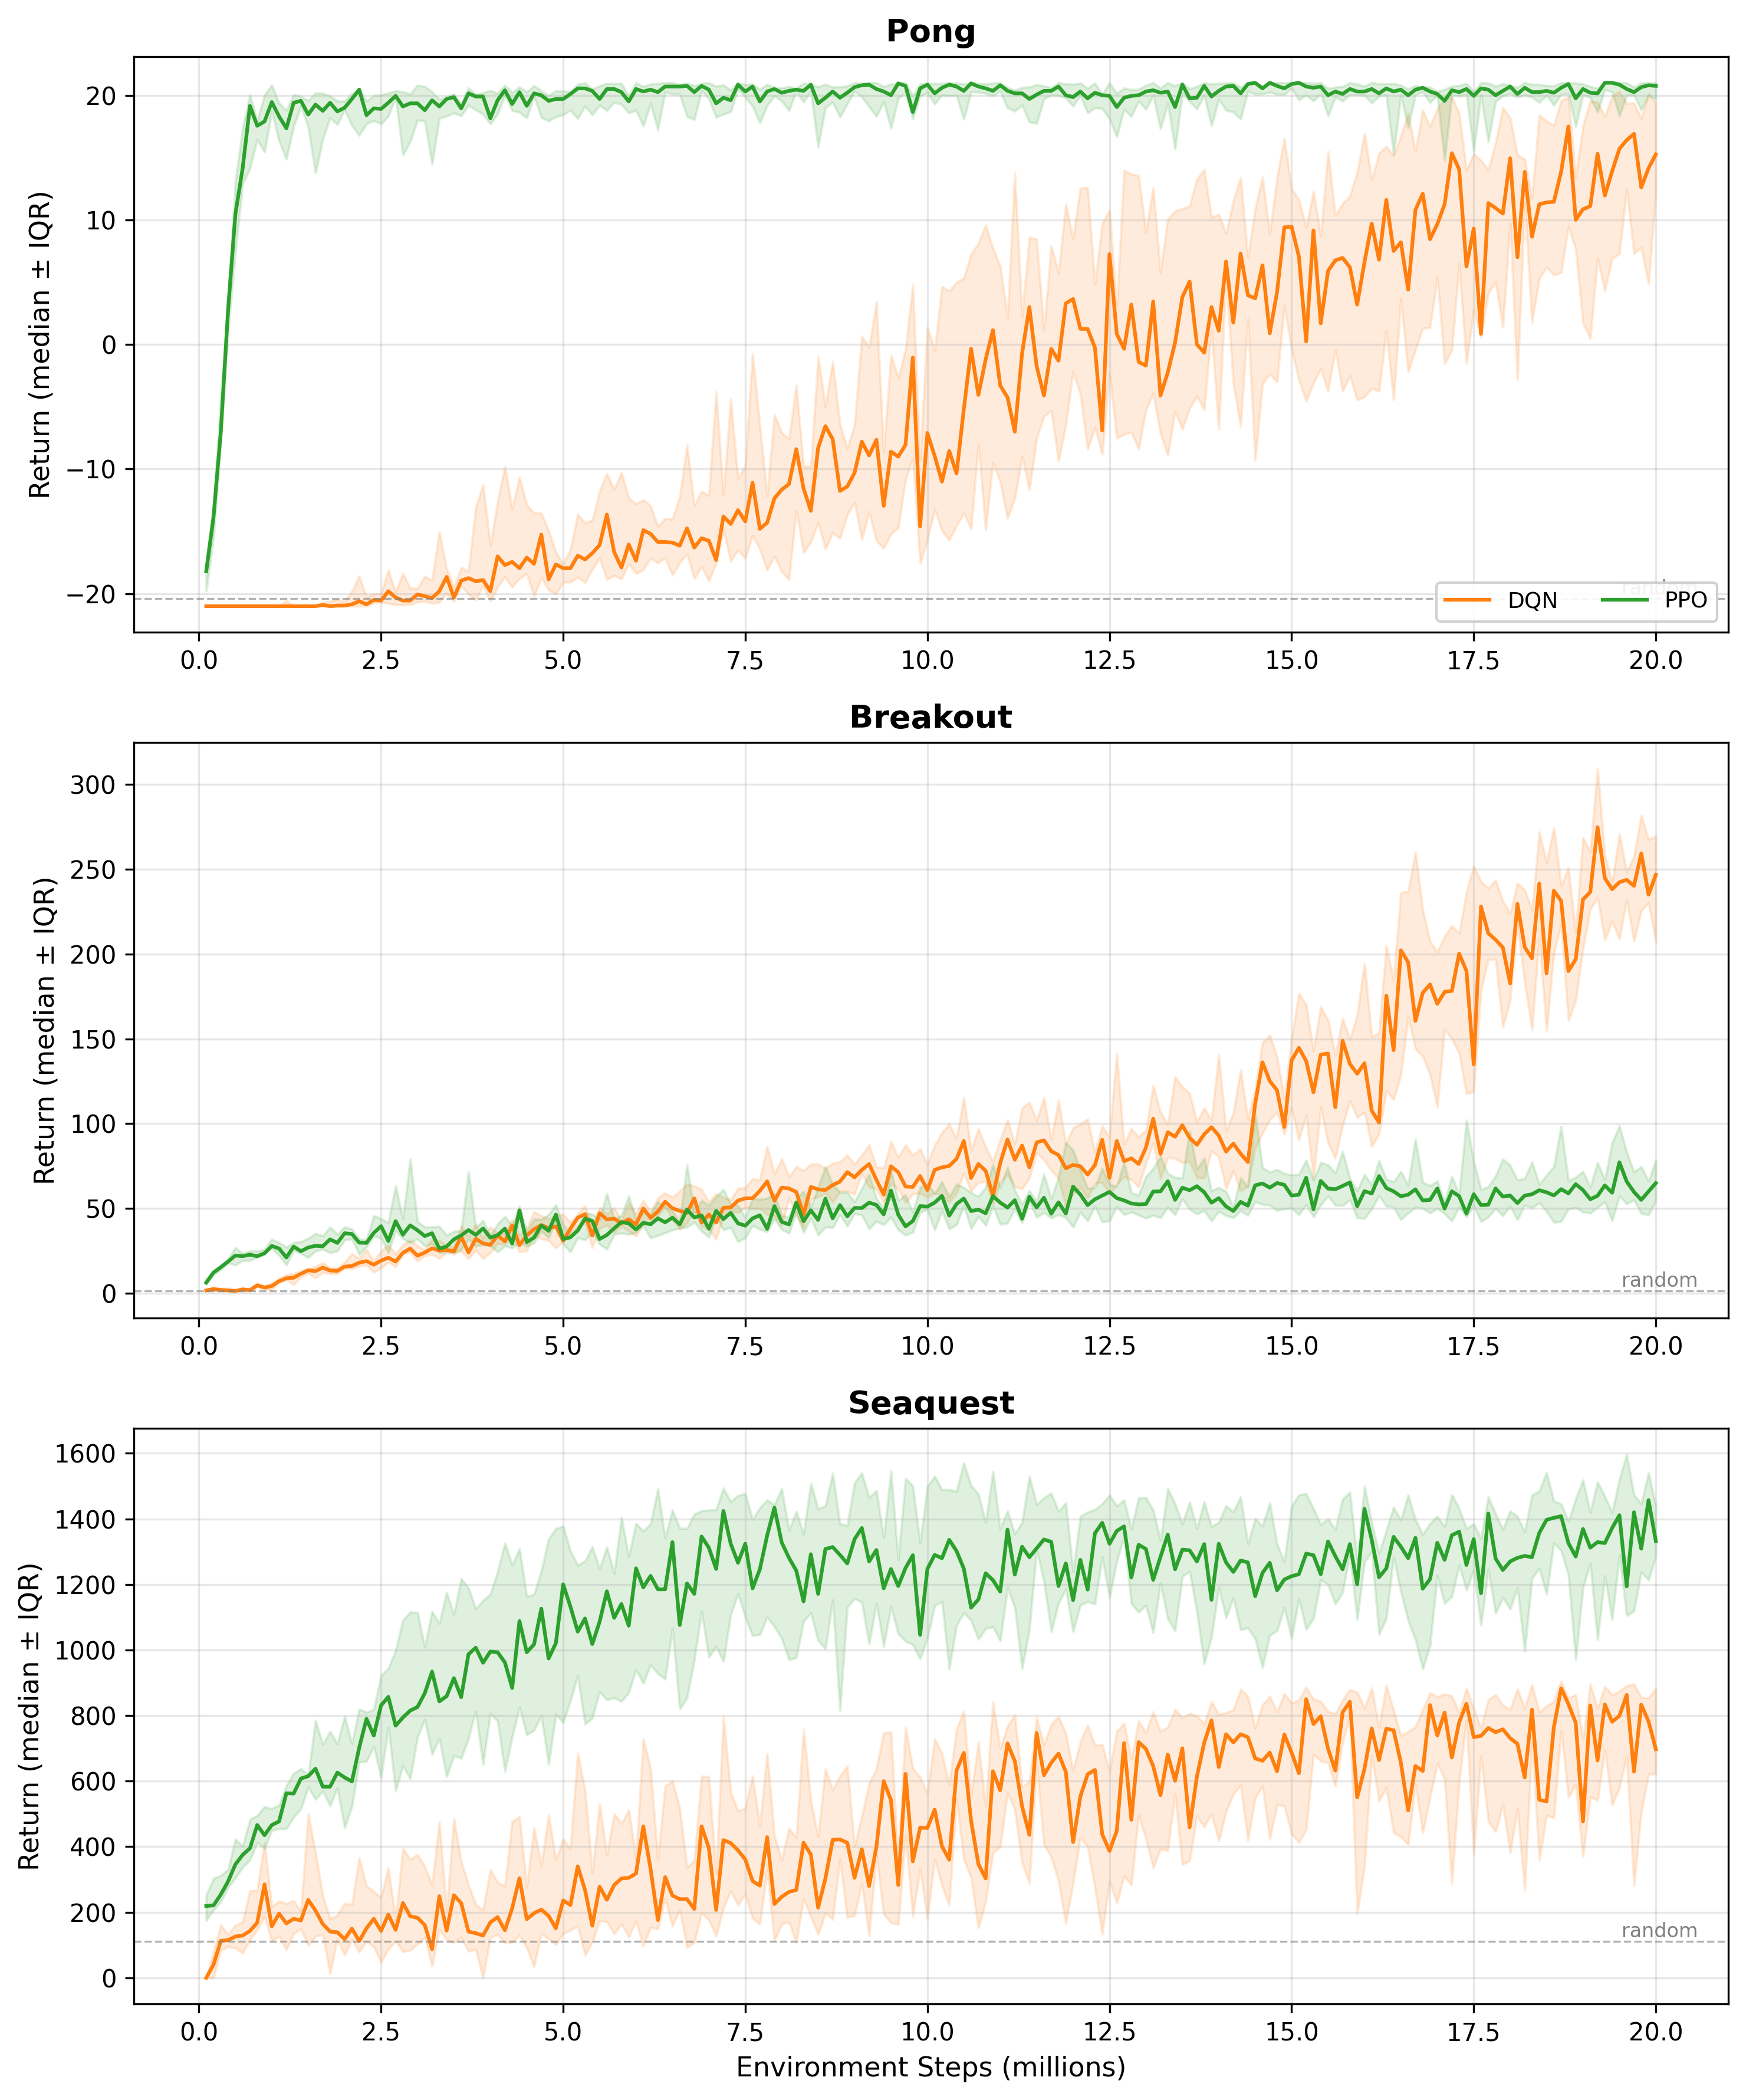
\includegraphics[width=\linewidth]{6_exp3_atari_extended/assets/combined_learning_curves.png}
  \caption[Combined learning curves: Pong, Breakout, Seaquest]{Combined normalised learning curves across Pong, Breakout, and Seaquest, 10 seeds per algorithm.}
  \label{fig:exp3-lc-combined}
\end{figure}

%% ------------------------------------------------------------------
\section{Score Distributions and Per-Seed Analysis}
\label{sec:exp3-score-dist}

Figures~\ref{fig:exp3-score-dist},~\ref{fig:exp3-heatmap}, and~\ref{fig:exp3-boxswarm} provide three complementary views. DQN scores are concentrated in the mid-range across all three environments. PPO is bimodal, with Pong and Seaquest seeds near their normalised ceilings and Breakout seeds near the floor.

\begin{figure}[htbp!]
  \centering
  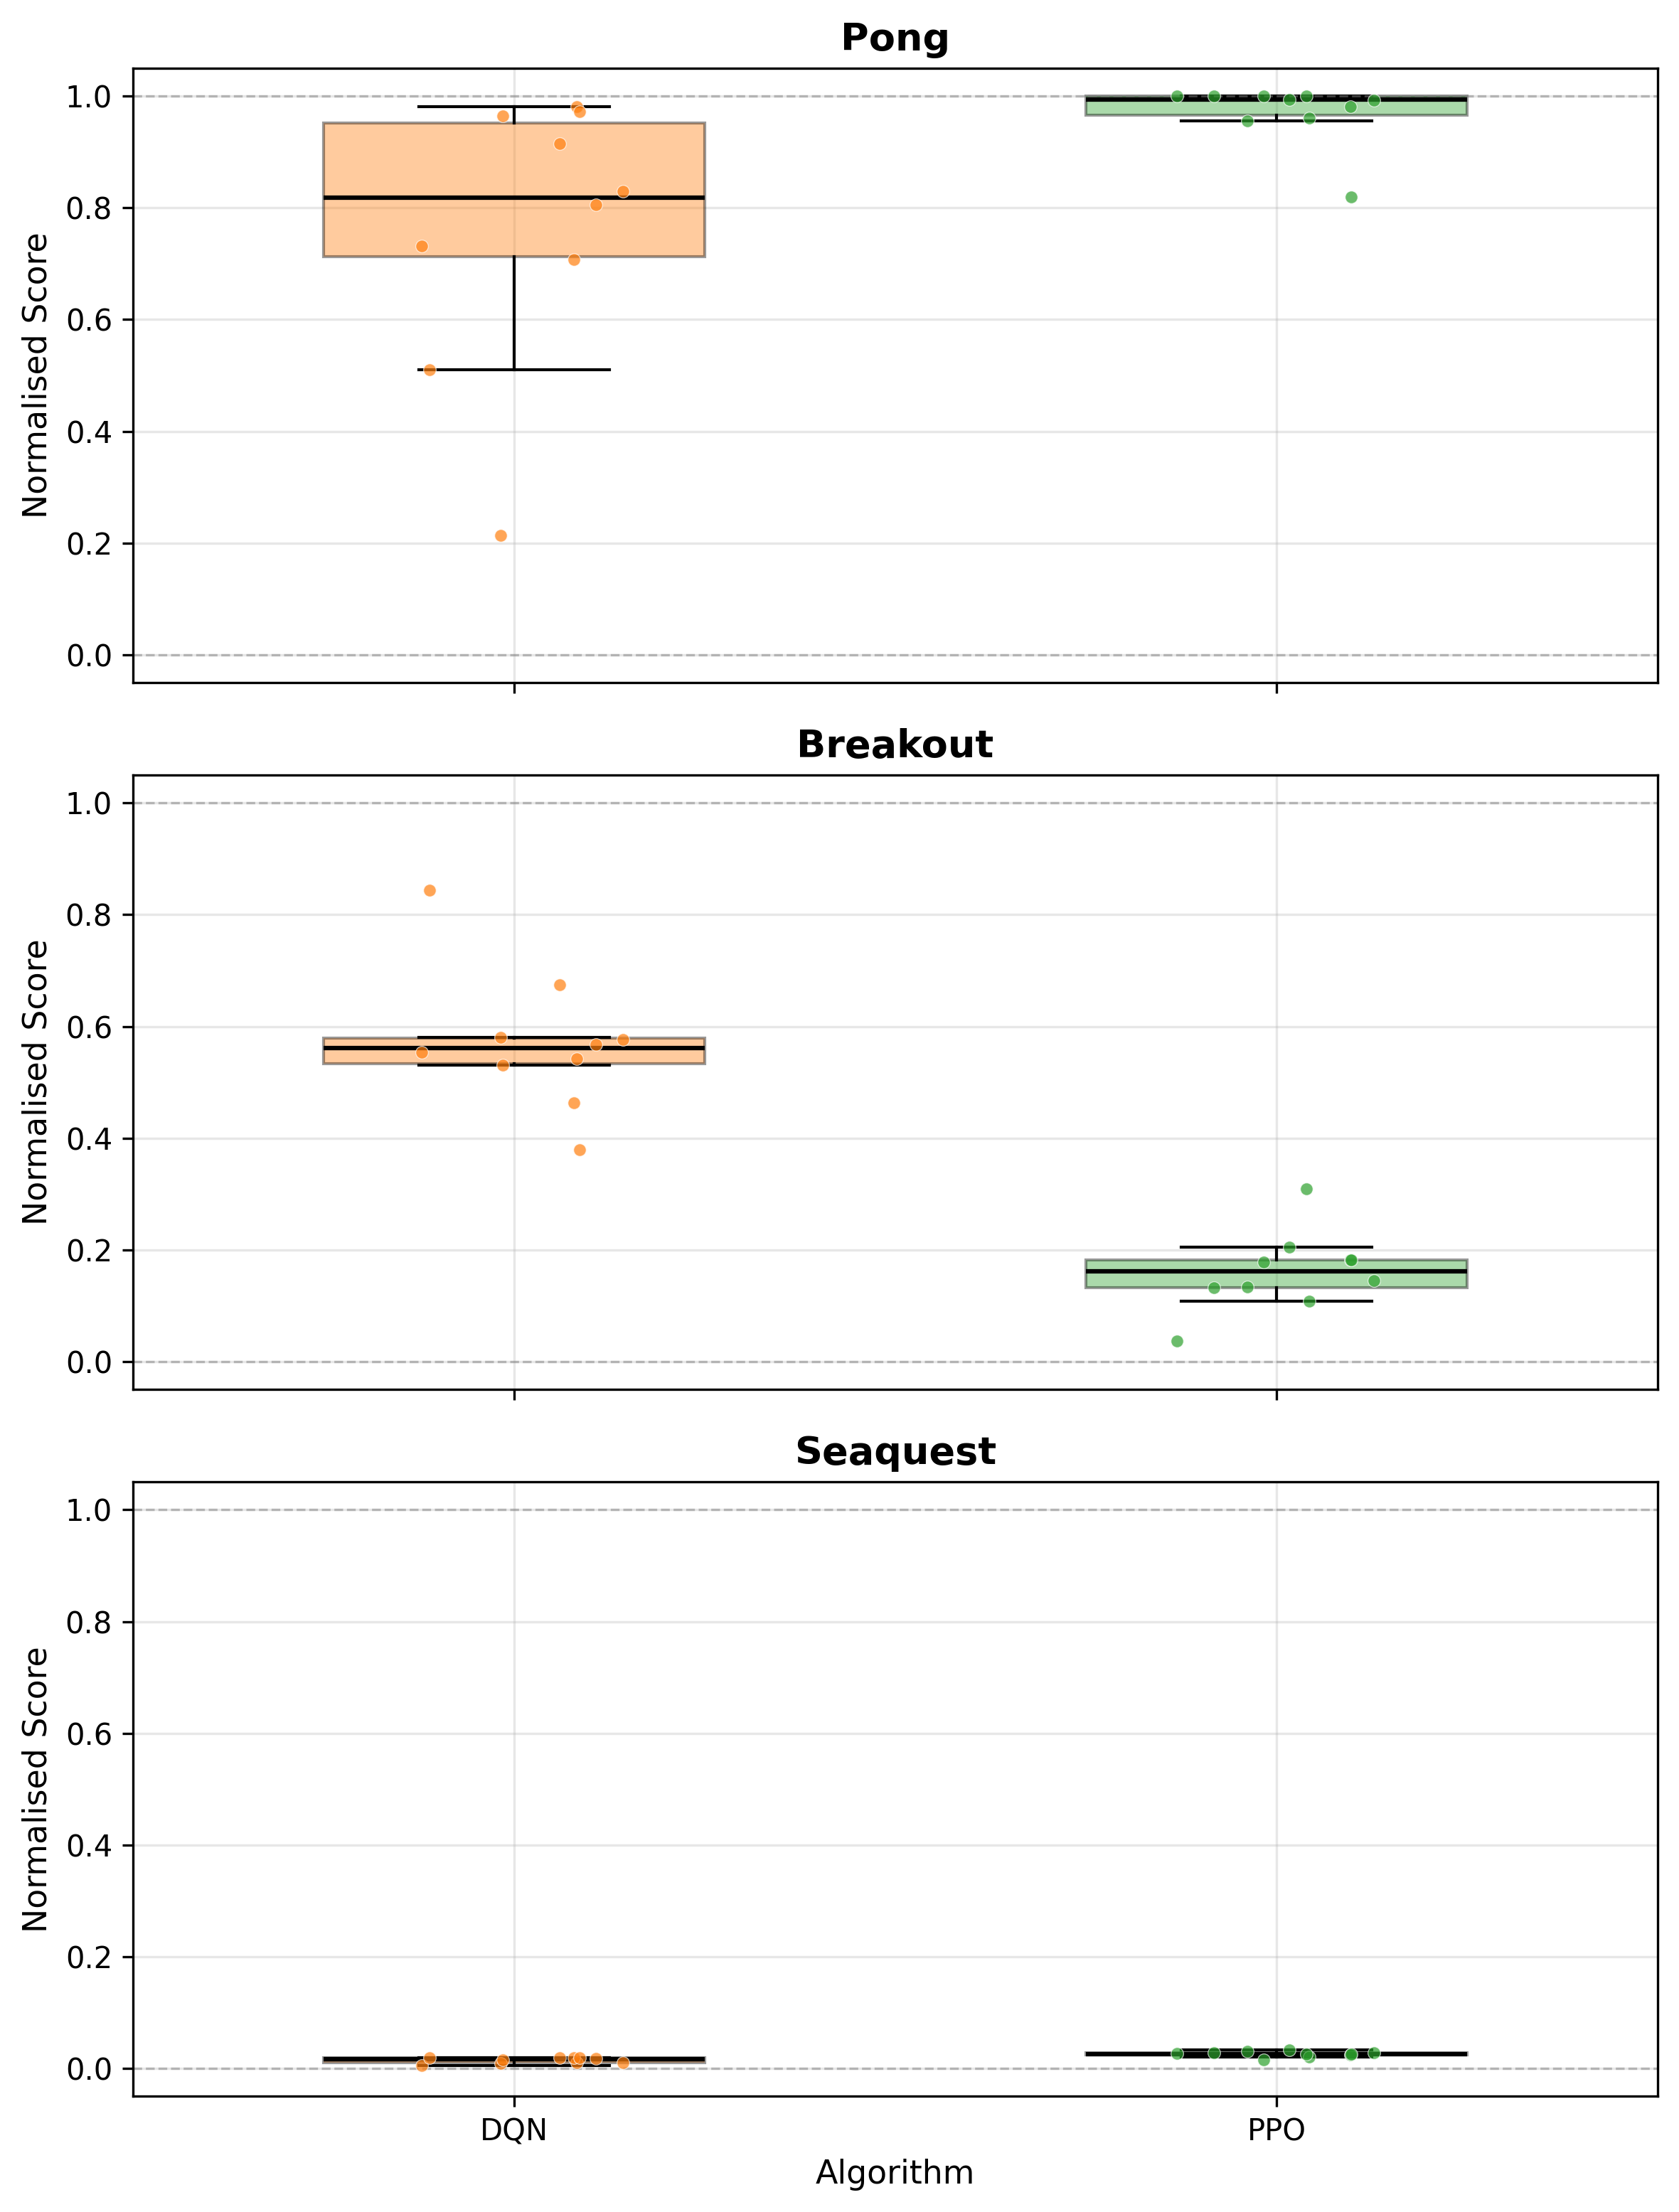
\includegraphics[width=\linewidth]{6_exp3_atari_extended/assets/score_distribution.png}
  \caption[Score distributions: Pong, Breakout, Seaquest]{Distribution of normalised final scores per environment. DQN is concentrated
           mid-range; PPO is bimodal (high on Pong and Seaquest, low on Breakout).}
  \label{fig:exp3-score-dist}
\end{figure}

\begin{figure}[htbp!]
  \centering
  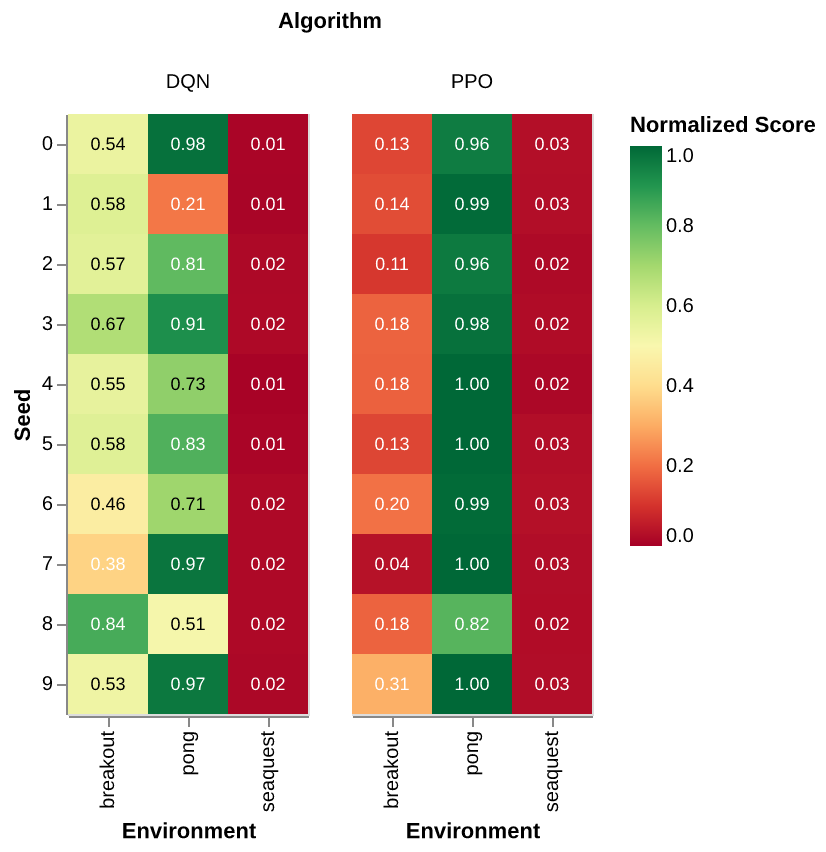
\includegraphics[width=\linewidth]{6_exp3_atari_extended/assets/per_seed_heatmap.png}
  \caption[Per-seed score heatmap: Pong, Breakout, Seaquest]{Heatmap of normalised final scores by seed (rows) and environment (columns).}
  \label{fig:exp3-heatmap}
\end{figure}

\begin{figure}[htbp!]
  \centering
  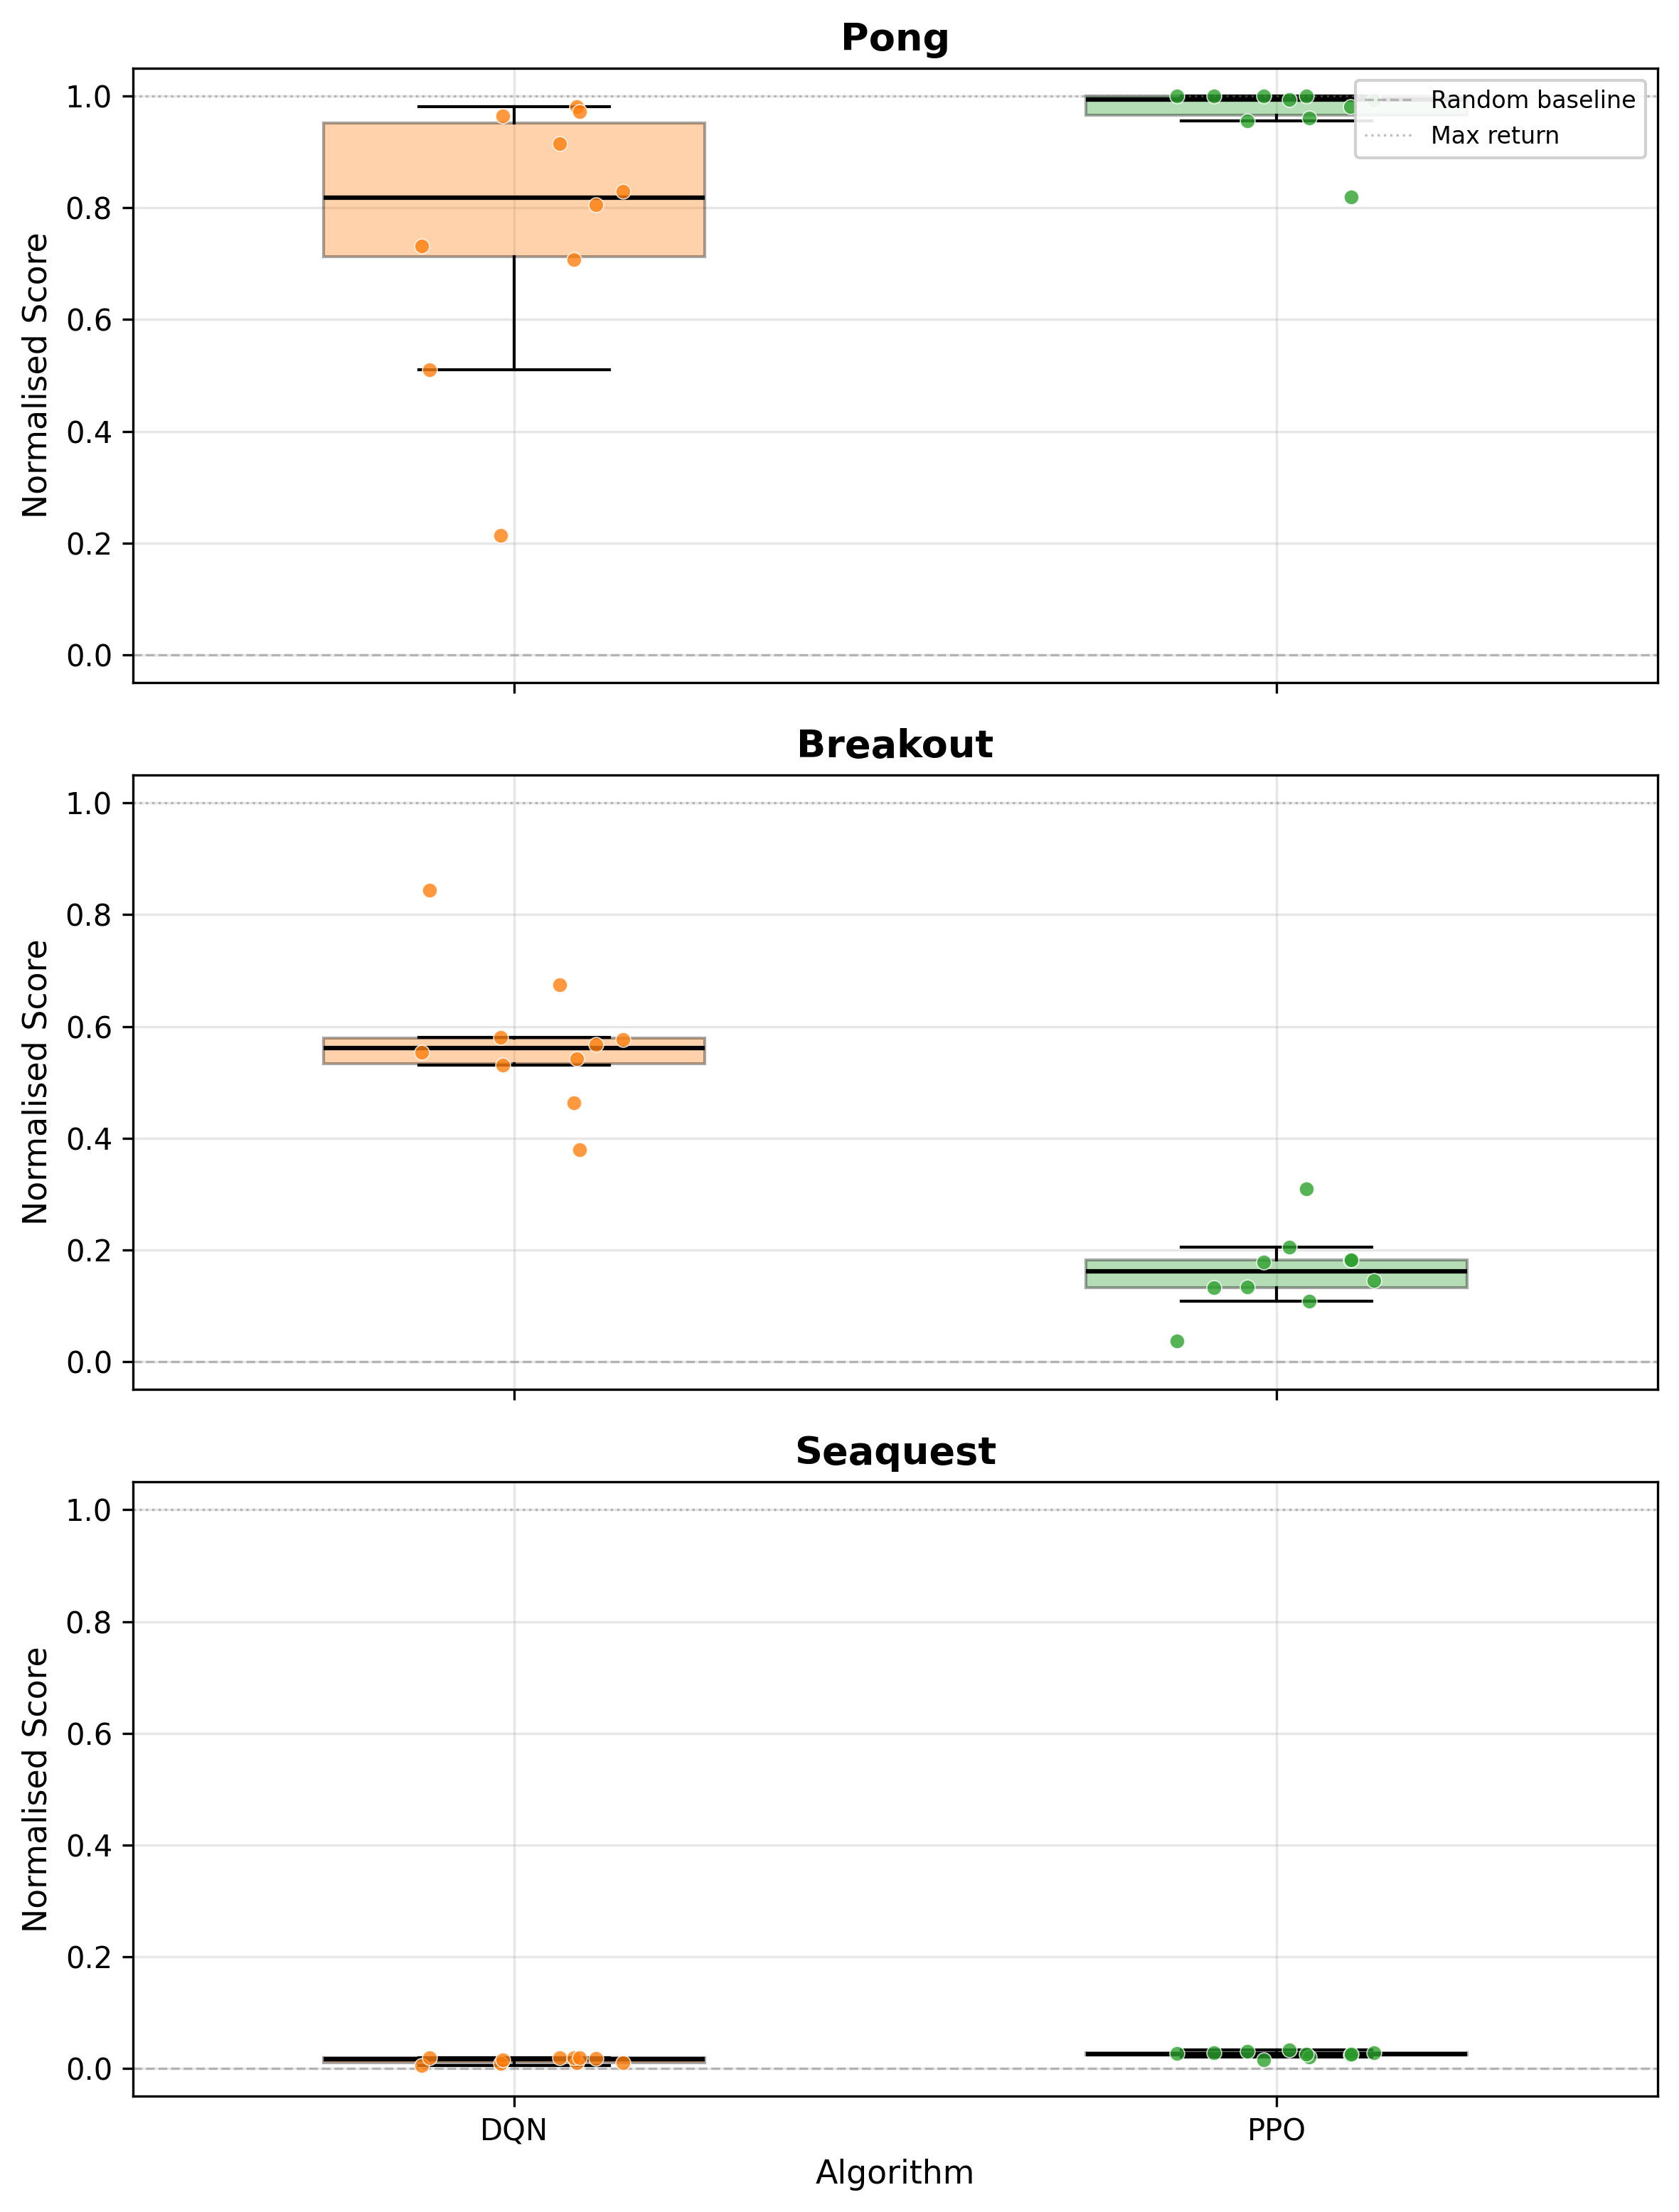
\includegraphics[width=\linewidth]{6_exp3_atari_extended/assets/per_seed_boxswarm.png}
  \caption[Per-seed score spread: Pong, Breakout, Seaquest]{Box-and-swarm plot of per-seed normalised scores across environments.}
  \label{fig:exp3-boxswarm}
\end{figure}

%% ------------------------------------------------------------------
\section{Cross-Environment Aggregate Results}
\label{sec:exp3-cross-env}

\subsection{Final Performance}
\label{sec:exp3-final-perf}

Table~\ref{tab:exp3-cross-env} and Figure~\ref{fig:exp3-final-perf} report the cross-environment aggregate metrics. DQN achieves a higher IQM (0.443, CI [0.369, 0.521]) than PPO (0.277, CI [0.247, 0.309]), with non-overlapping confidence intervals.

\begin{table}[htbp!]
\centering
\caption{Cross-environment aggregate metrics for Experiment~3 (normalised scores).}
\label{tab:exp3-cross-env}
\begin{tabular}{lcccc}
\toprule
\textbf{Algorithm} & \textbf{IQM} & \textbf{Mean} & \textbf{Median} & \textbf{Opt.\ Gap} \\
\midrule
DQN & $0.443\;[0.369,\;0.521]$ & --- & --- & $0.550\;[0.500,\;0.607]$ \\
PPO & $0.277\;[0.247,\;0.309]$ & --- & --- & $0.614\;[0.597,\;0.632]$ \\
\bottomrule
\end{tabular}
\end{table}

\begin{figure}[htbp!]
  \centering
  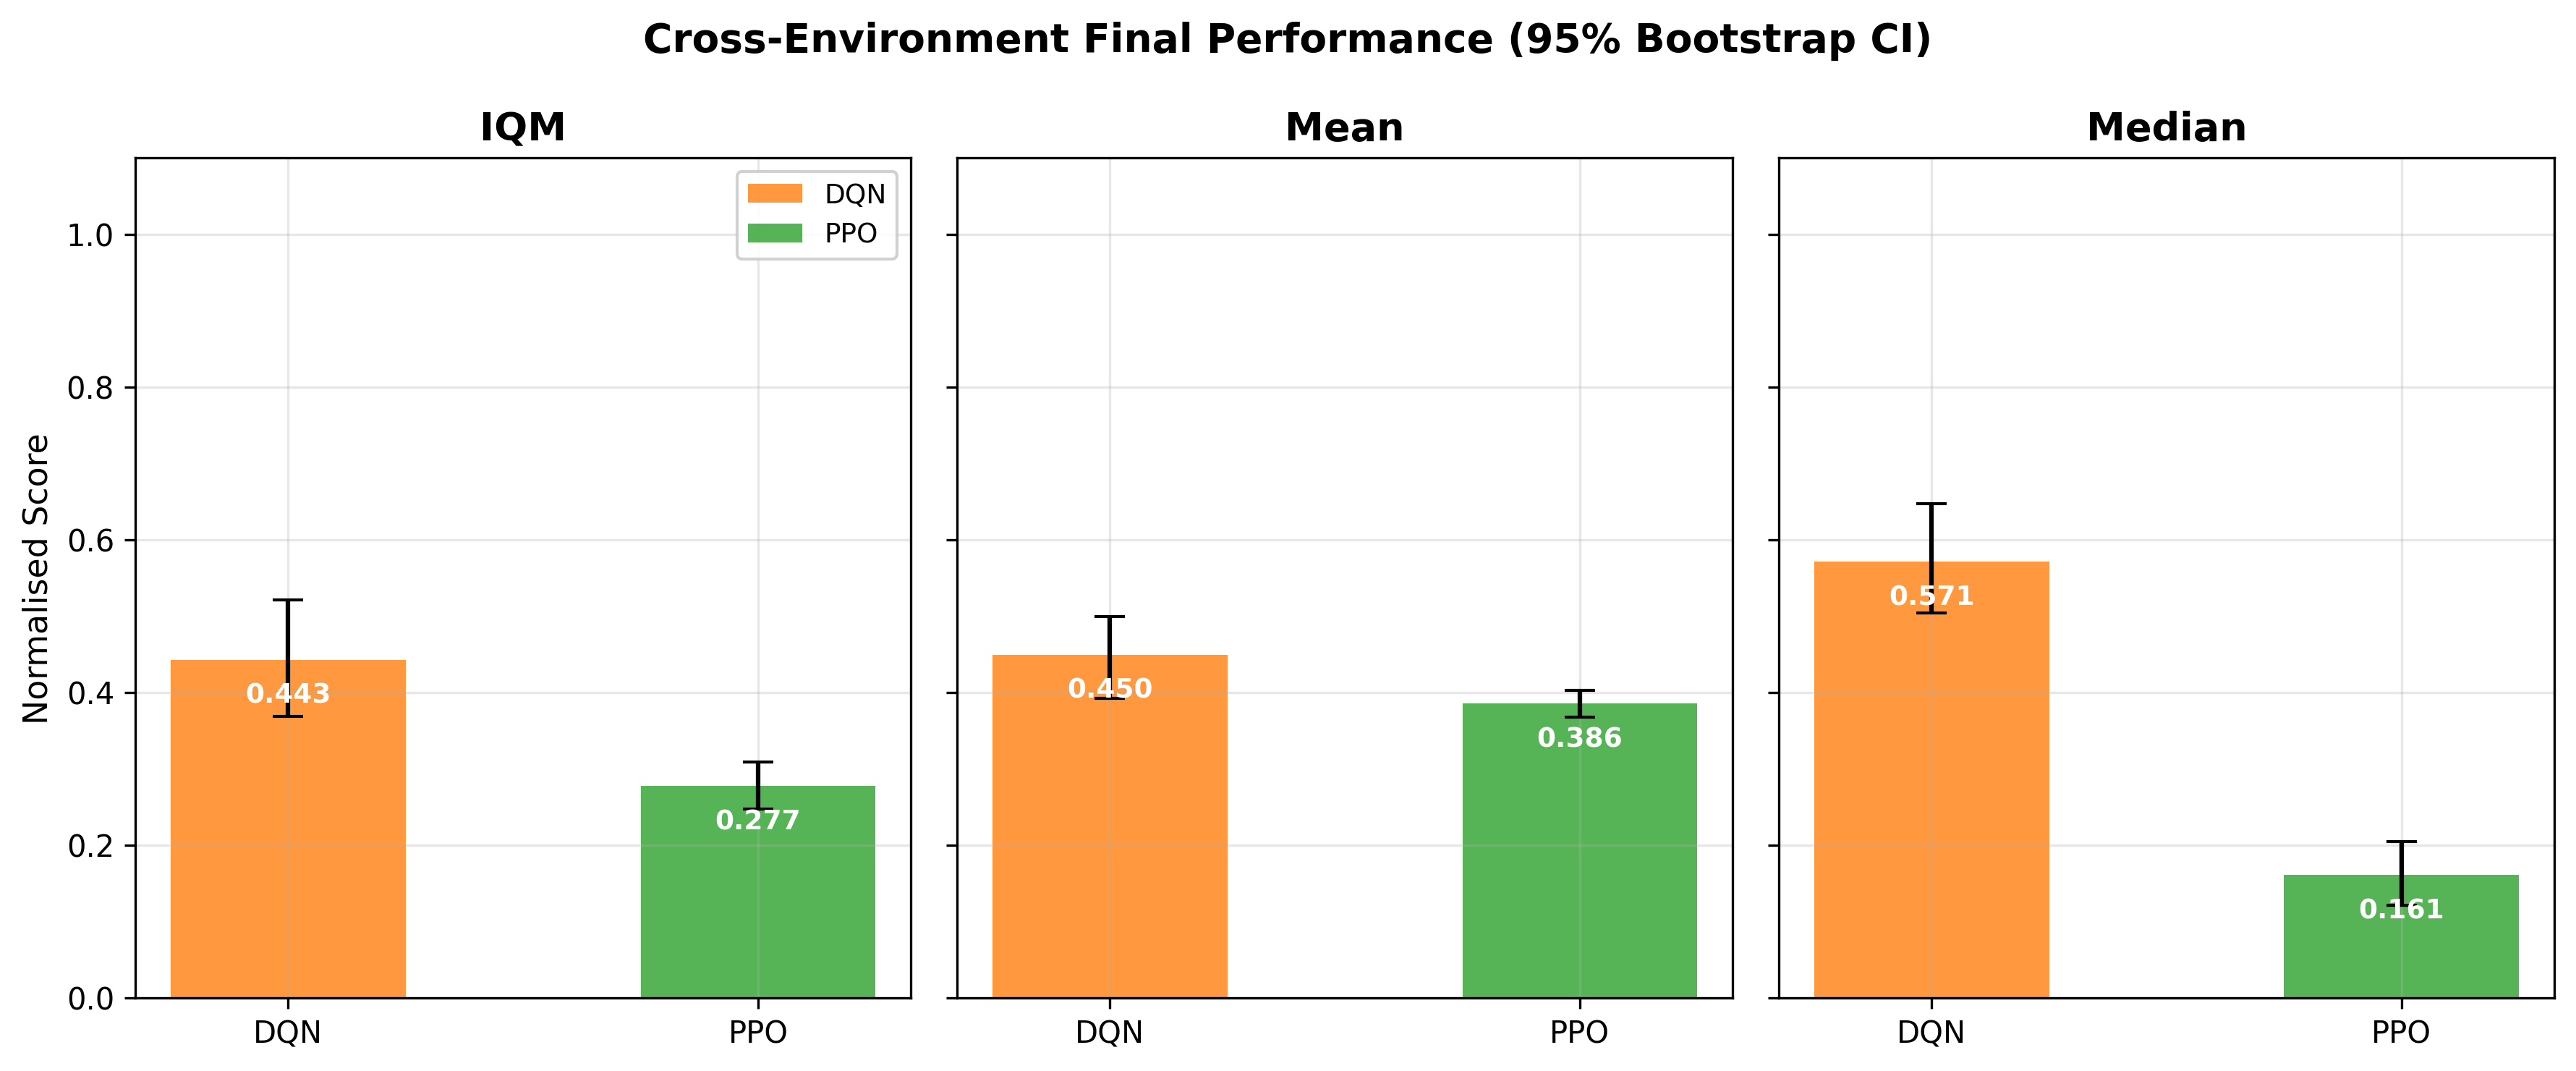
\includegraphics[width=\linewidth]{6_exp3_atari_extended/assets/final_performance.png}
  \caption[Cross-environment IQM: Pong, Breakout, Seaquest]{Cross-environment IQM, mean, and median with 95\% bootstrap CIs.
           DQN IQM 0.443 vs PPO 0.277 (non-overlapping CIs).}
  \label{fig:exp3-final-perf}
\end{figure}

\subsection{Performance Profile and Optimality Gap}
\label{sec:exp3-profile-gap}

\begin{figure}[htbp!]
  \centering
  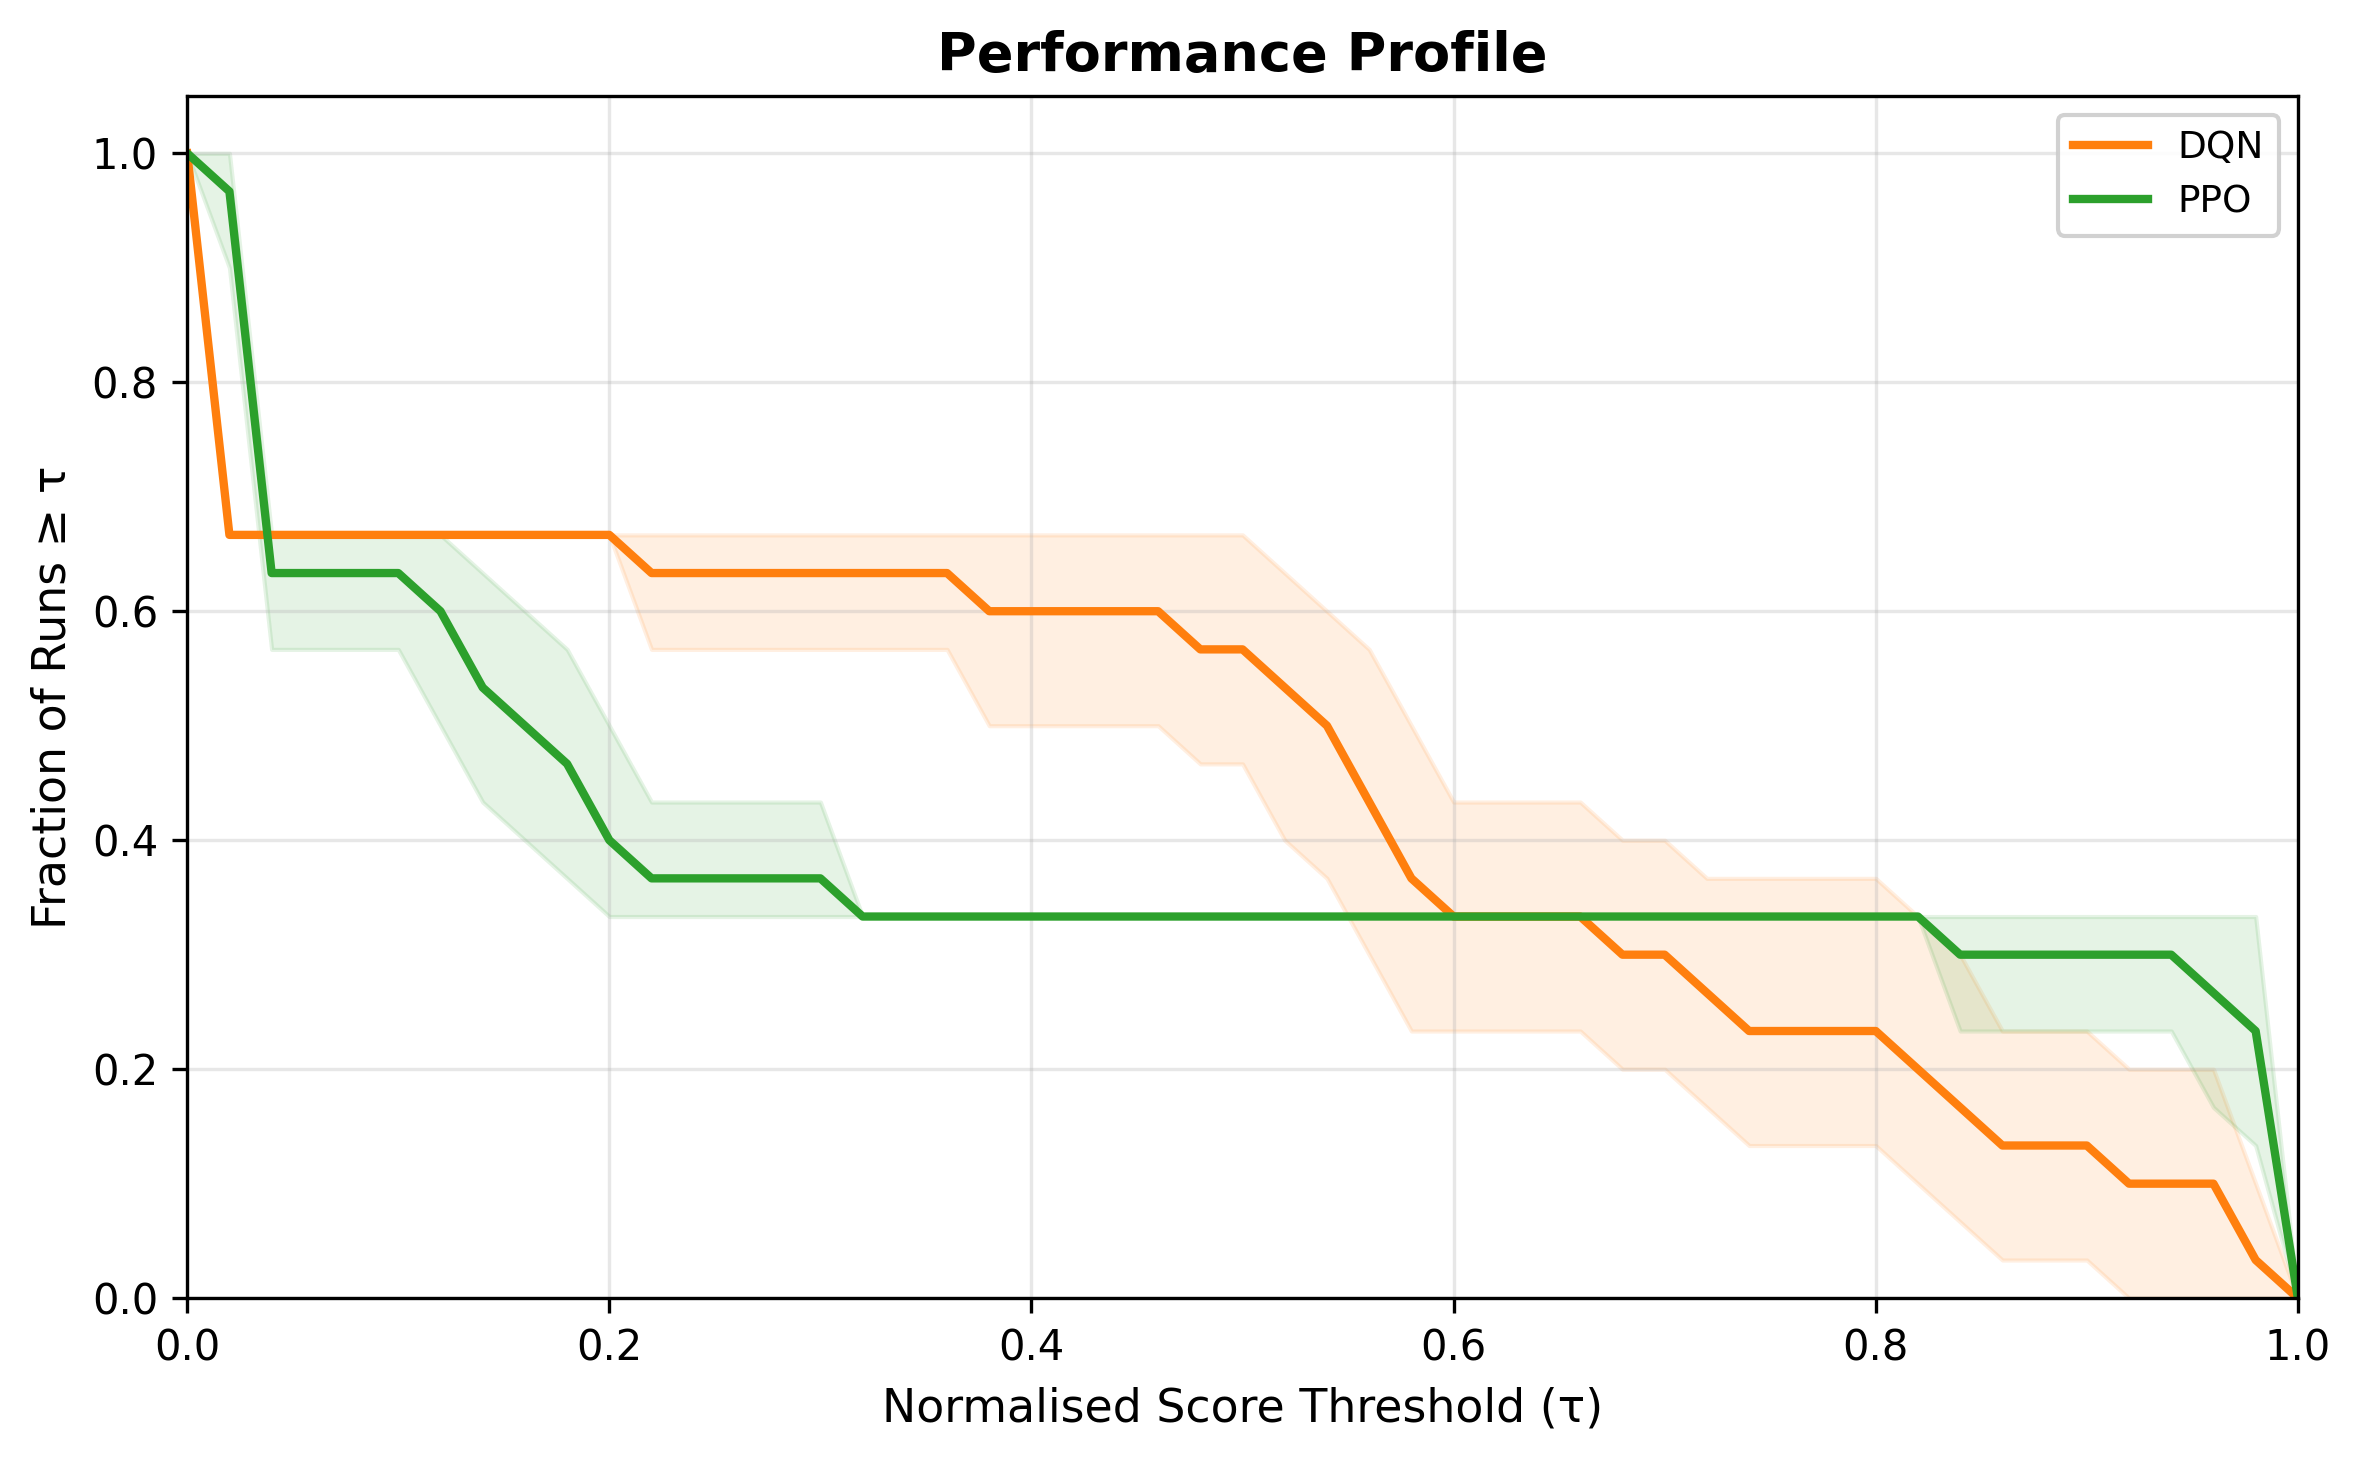
\includegraphics[width=\linewidth]{6_exp3_atari_extended/assets/performance_profile.png}
  \caption{Performance profiles with 95\% bootstrap CIs.}
  \label{fig:exp3-perf-profile}
\end{figure}

\begin{figure}[htbp!]
  \centering
  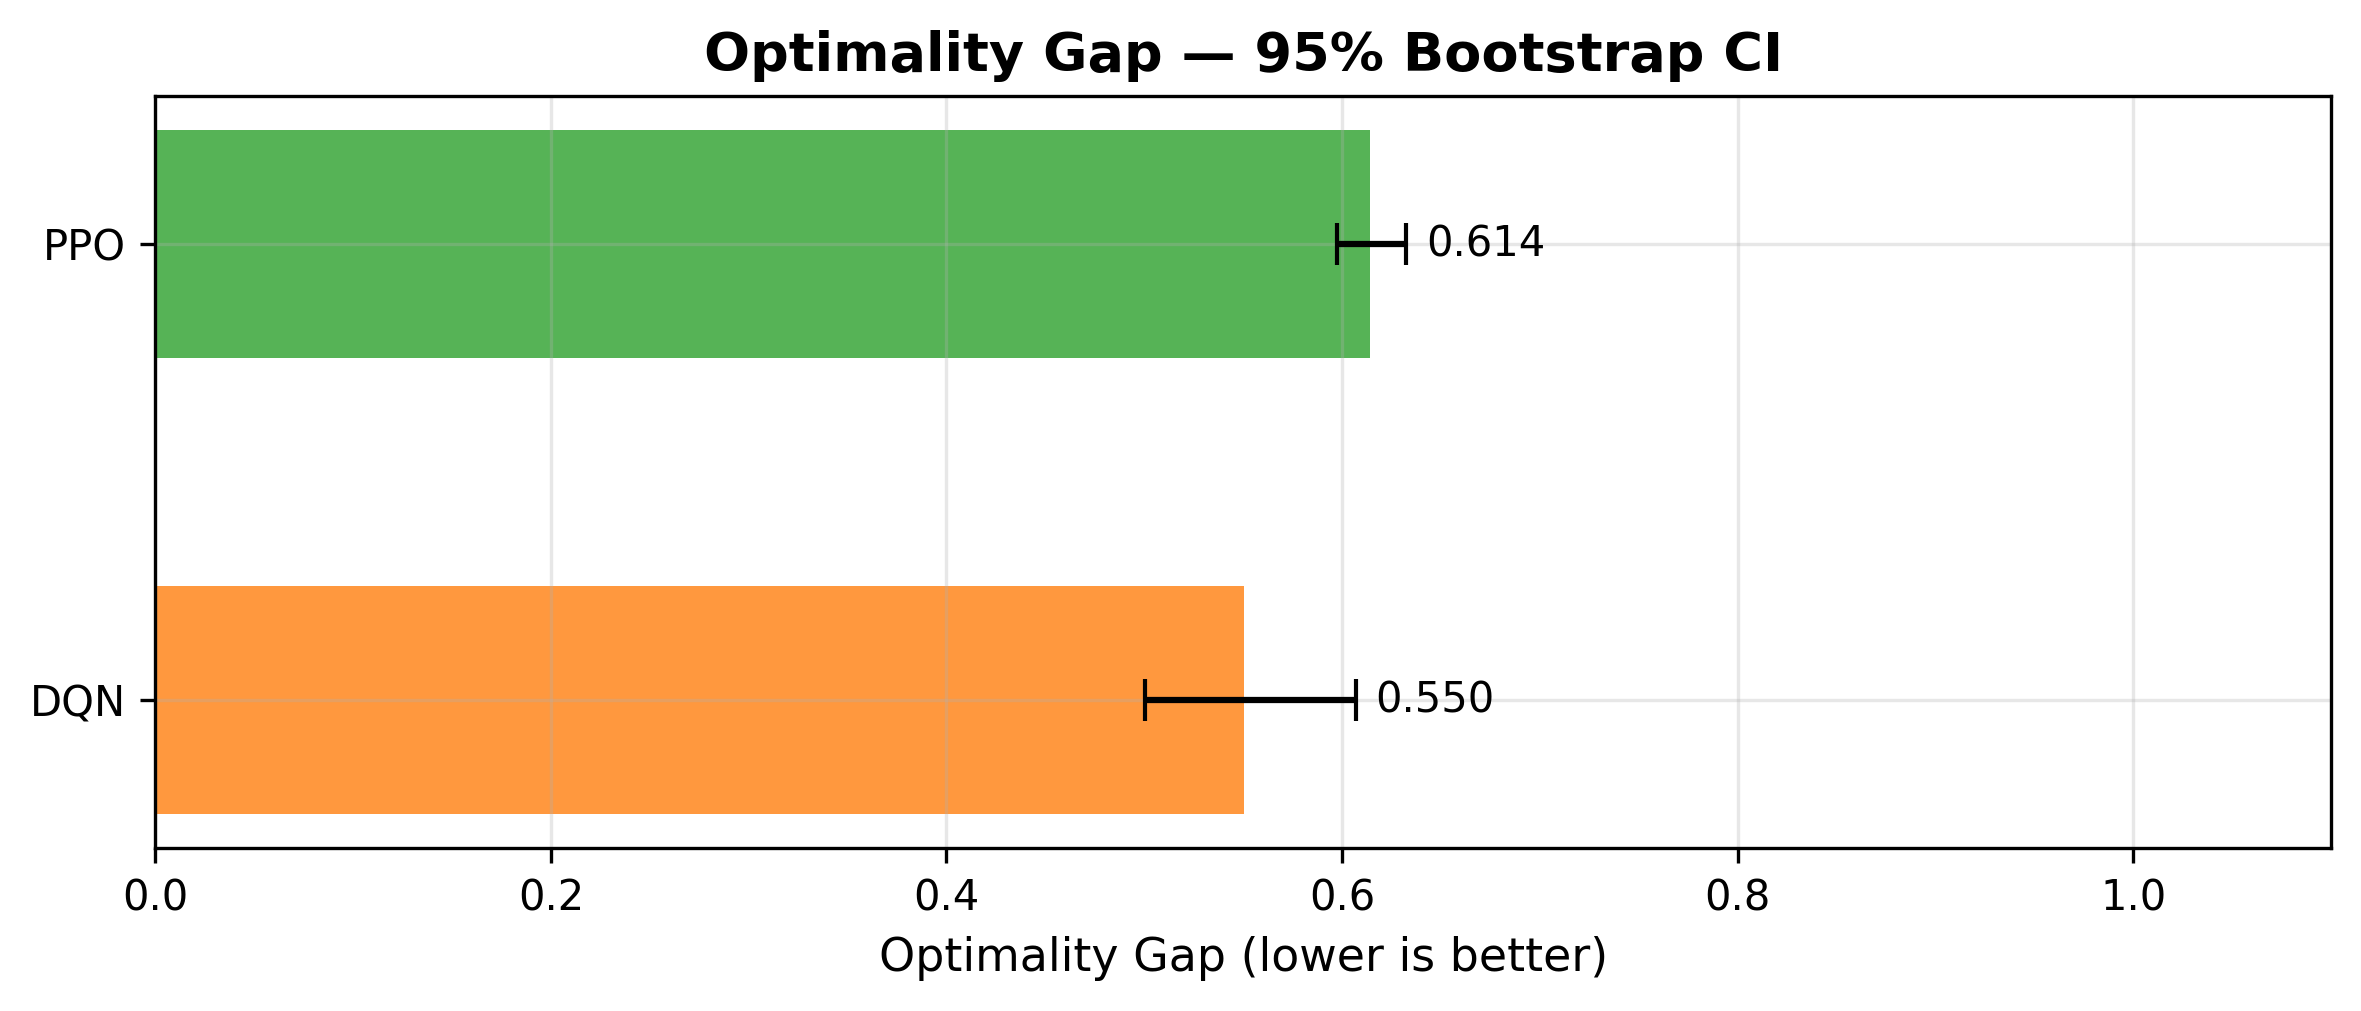
\includegraphics[width=0.7\linewidth]{6_exp3_atari_extended/assets/optimality_gap.png}
  \caption[Optimality gap: Pong, Breakout, Seaquest]{Optimality gap. Lower is better. DQN 0.550 (CI [0.500, 0.607]),
           PPO 0.614 (CI [0.597, 0.632]).}
  \label{fig:exp3-opt-gap}
\end{figure}

\subsection{Pairwise Probability of Improvement}
\label{sec:exp3-poi}

Figure~\ref{fig:exp3-poi} shows that $P(\text{DQN}>\text{PPO}) = 0.393$, meaning a randomly chosen PPO run is \emph{more likely} to beat a randomly chosen DQN run pairwise --- the opposite of what the IQM says. Both numbers come from the same score matrix; the contradiction is not an error and is discussed in Section~\ref{sec:exp3-discussion}.

\begin{figure}[htbp!]
  \centering
  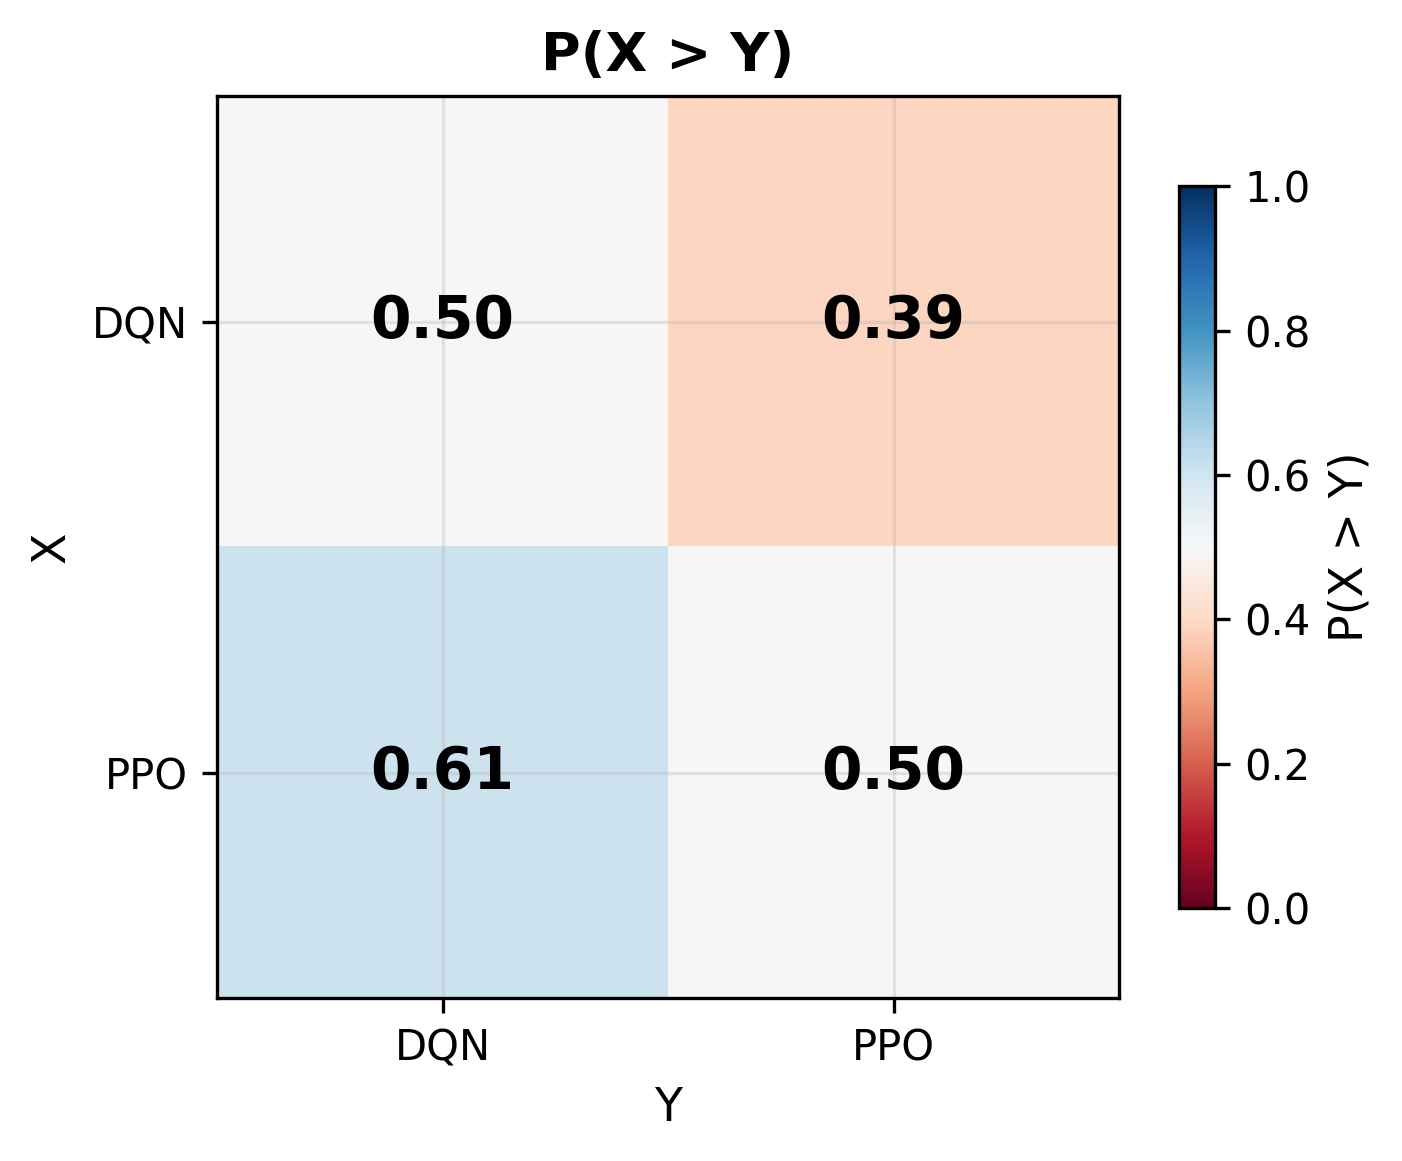
\includegraphics[width=0.6\linewidth]{6_exp3_atari_extended/assets/poi_heatmap.png}
  \caption[Probability of improvement: DQN vs PPO, 3 environments]{Pairwise probability of improvement: $P(\text{DQN}>\text{PPO}) = 0.393$.
           PPO wins a majority of pairwise comparisons despite a lower IQM.}
  \label{fig:exp3-poi}
\end{figure}

%% ------------------------------------------------------------------
\section{Sample Efficiency}
\label{sec:exp3-sample-eff}

\begin{figure}[htbp!]
  \centering
  \begin{subfigure}[b]{0.48\linewidth}
    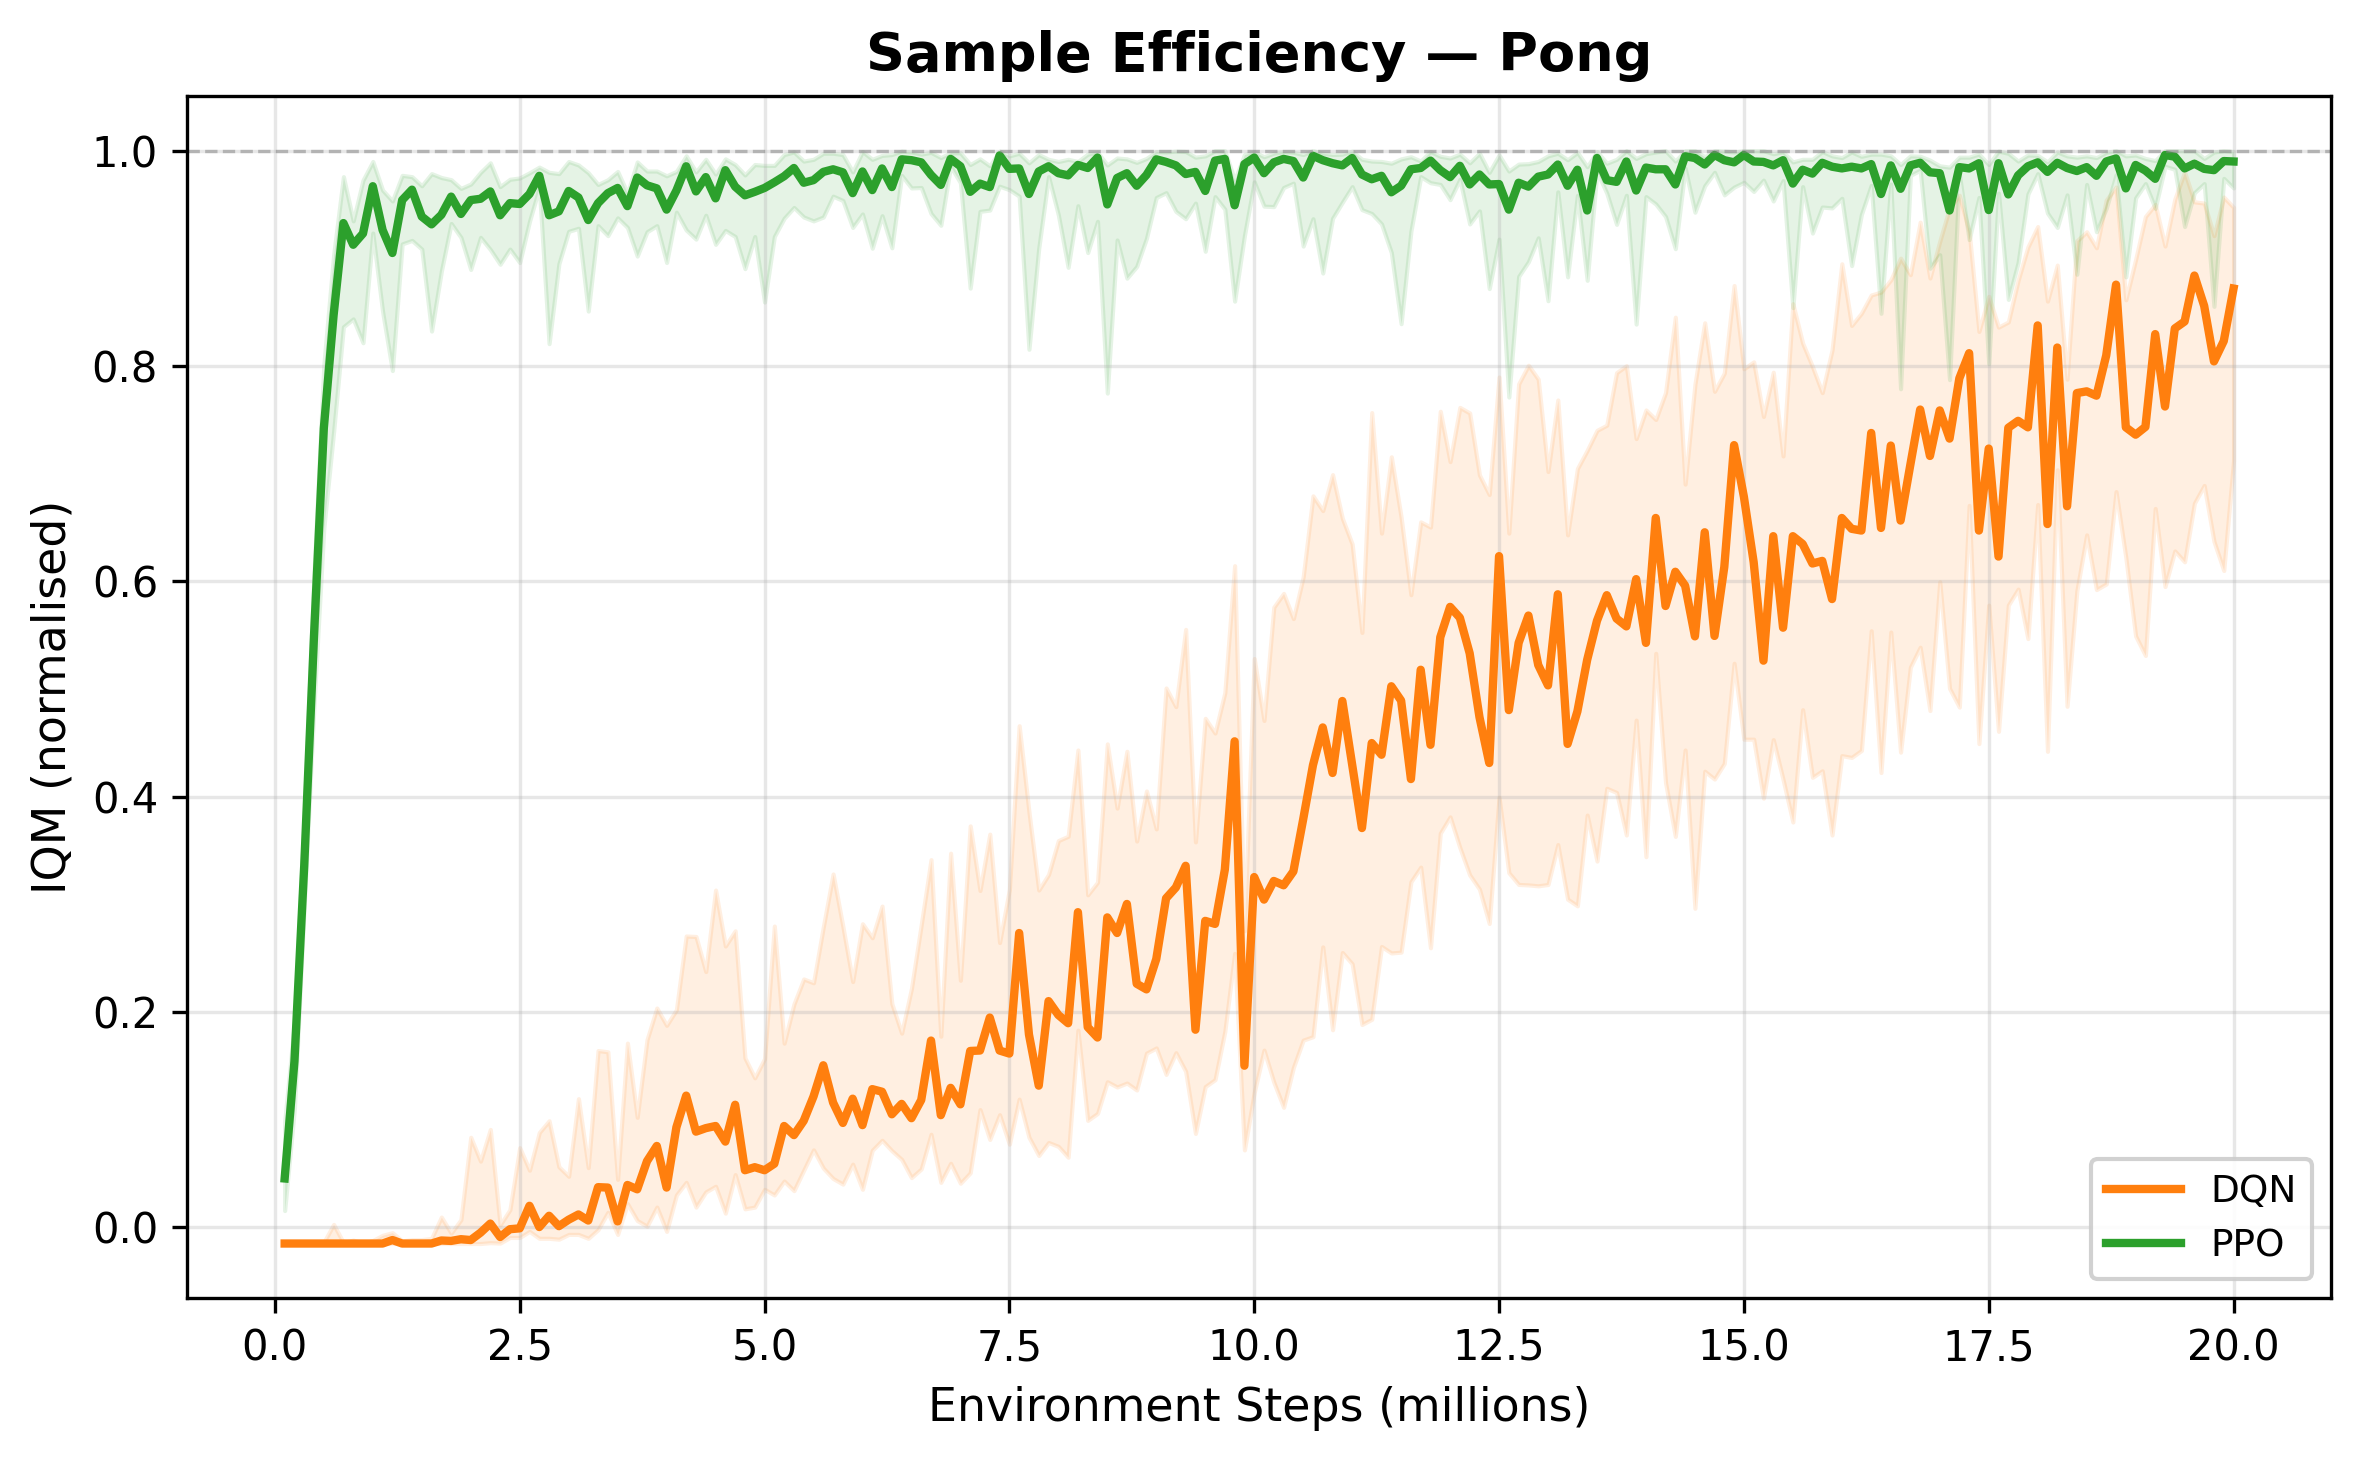
\includegraphics[width=\linewidth]{6_exp3_atari_extended/assets/sample_efficiency_pong.png}
    \caption{Pong}
  \end{subfigure}
  \hfill
  \begin{subfigure}[b]{0.48\linewidth}
    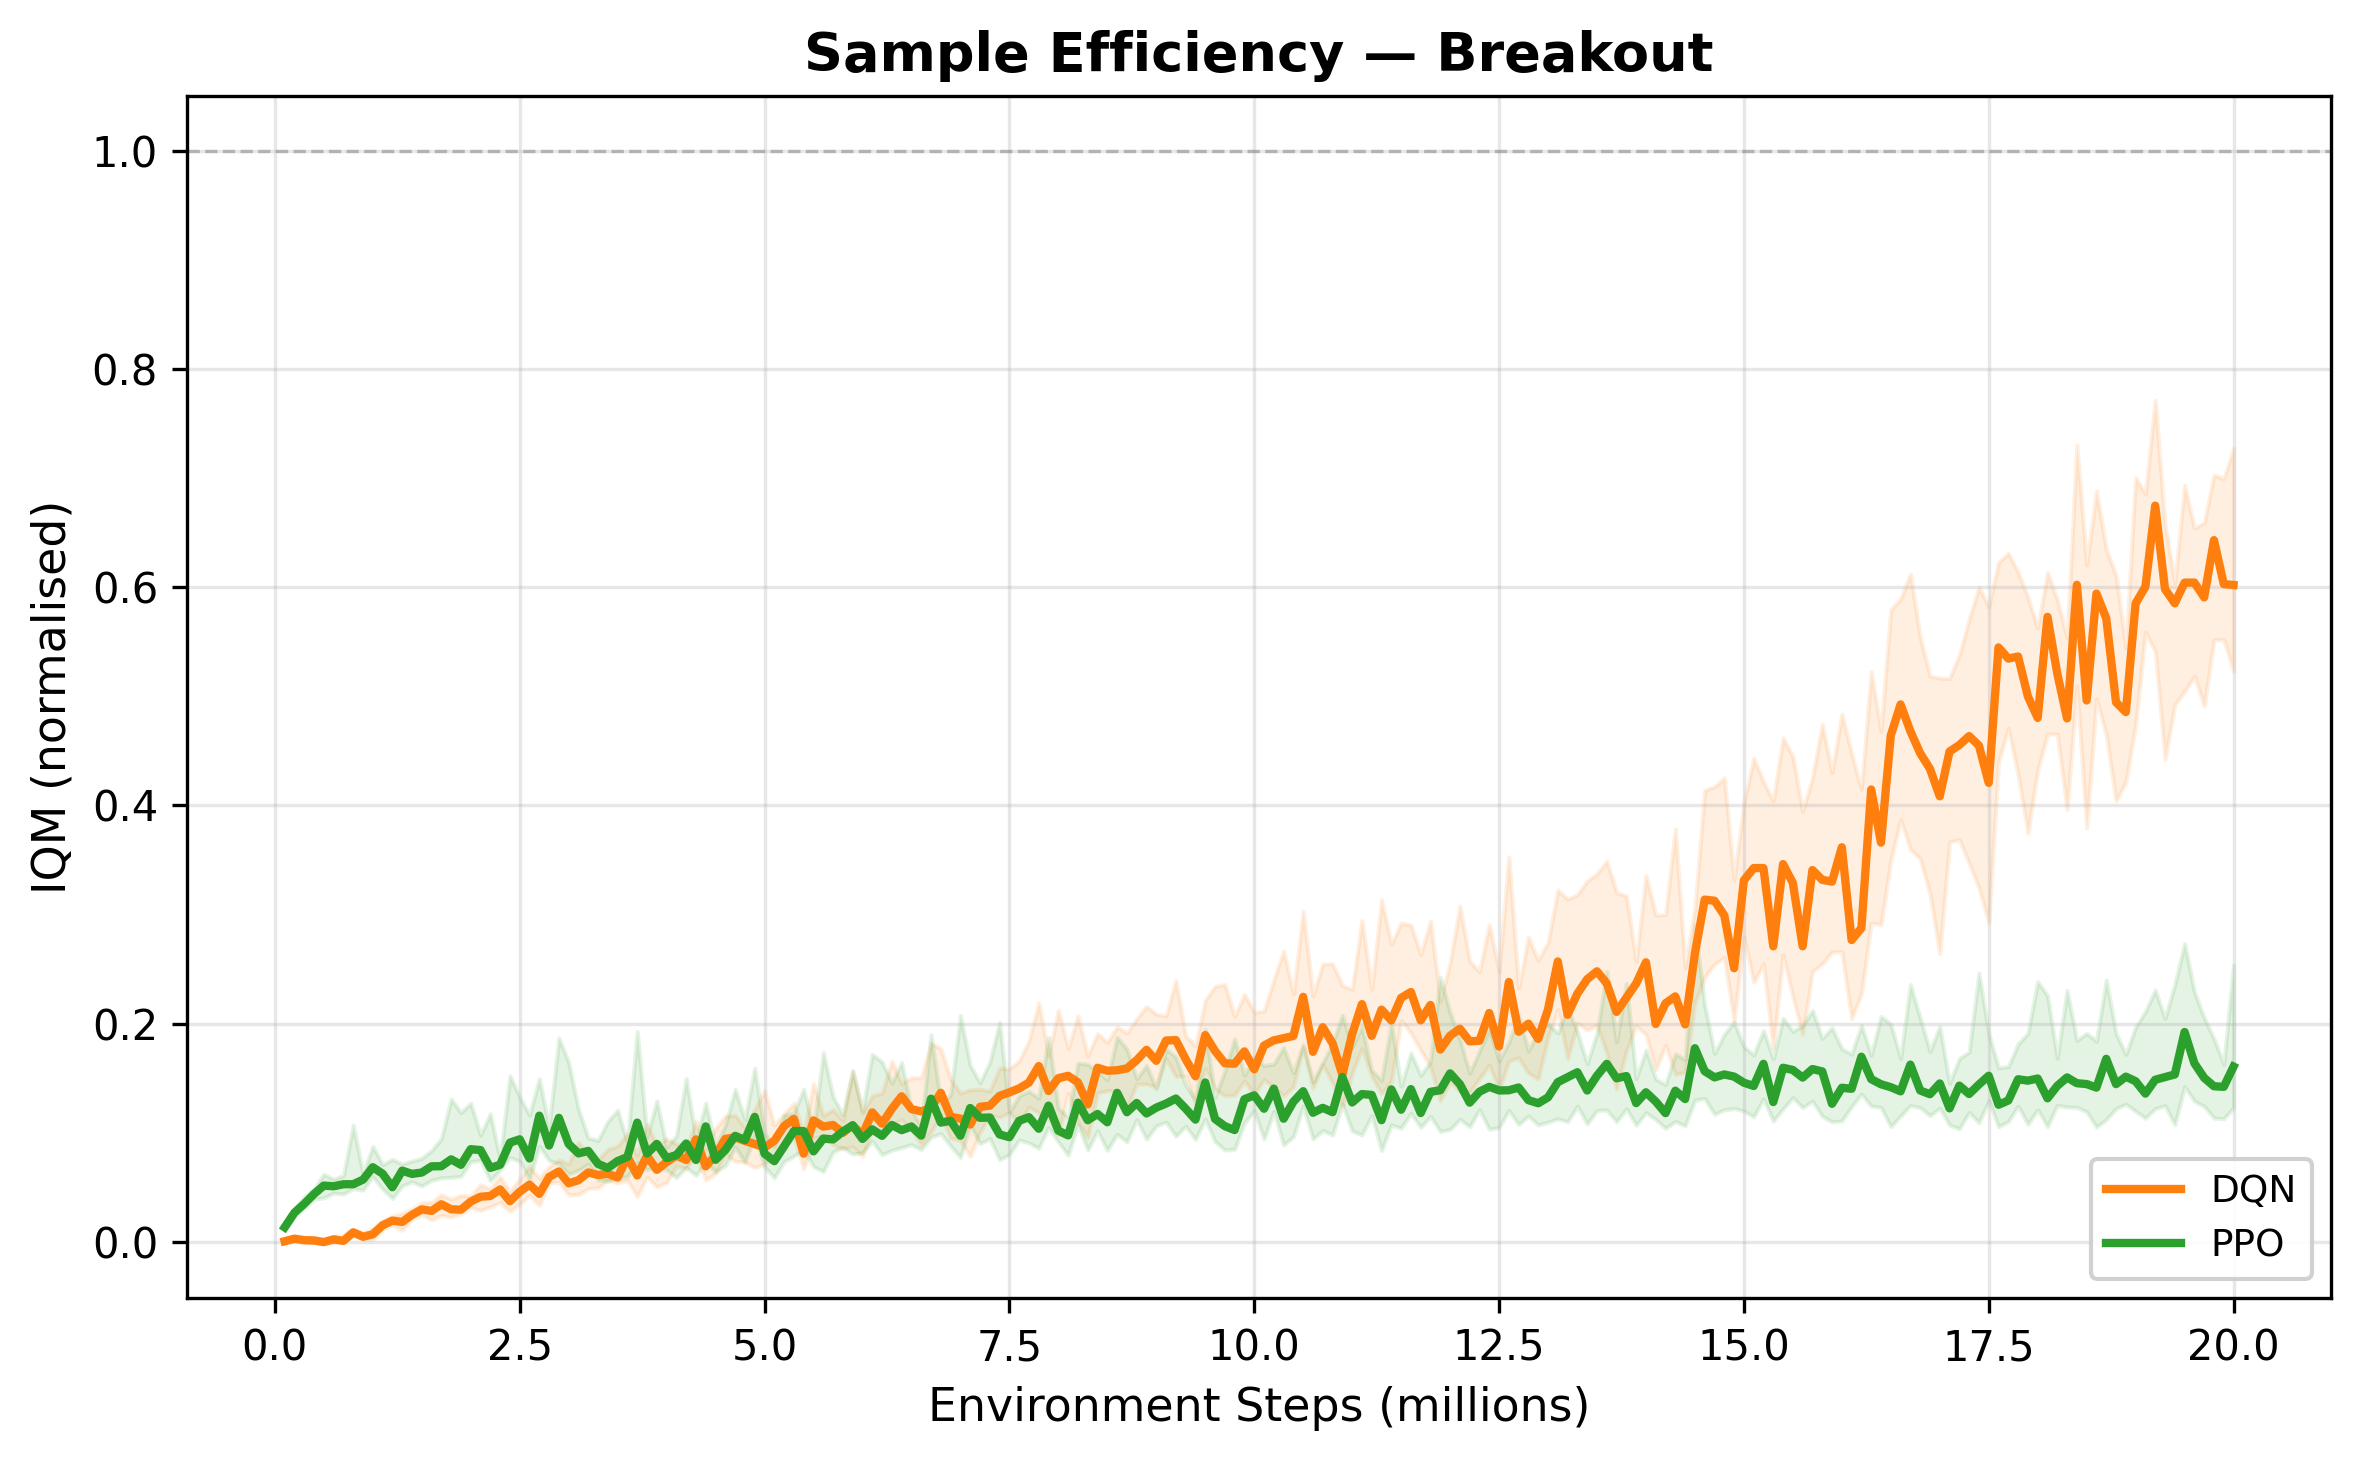
\includegraphics[width=\linewidth]{6_exp3_atari_extended/assets/sample_efficiency_breakout.png}
    \caption{Breakout}
  \end{subfigure}

  \vspace{0.5em}
  \begin{subfigure}[b]{0.48\linewidth}
    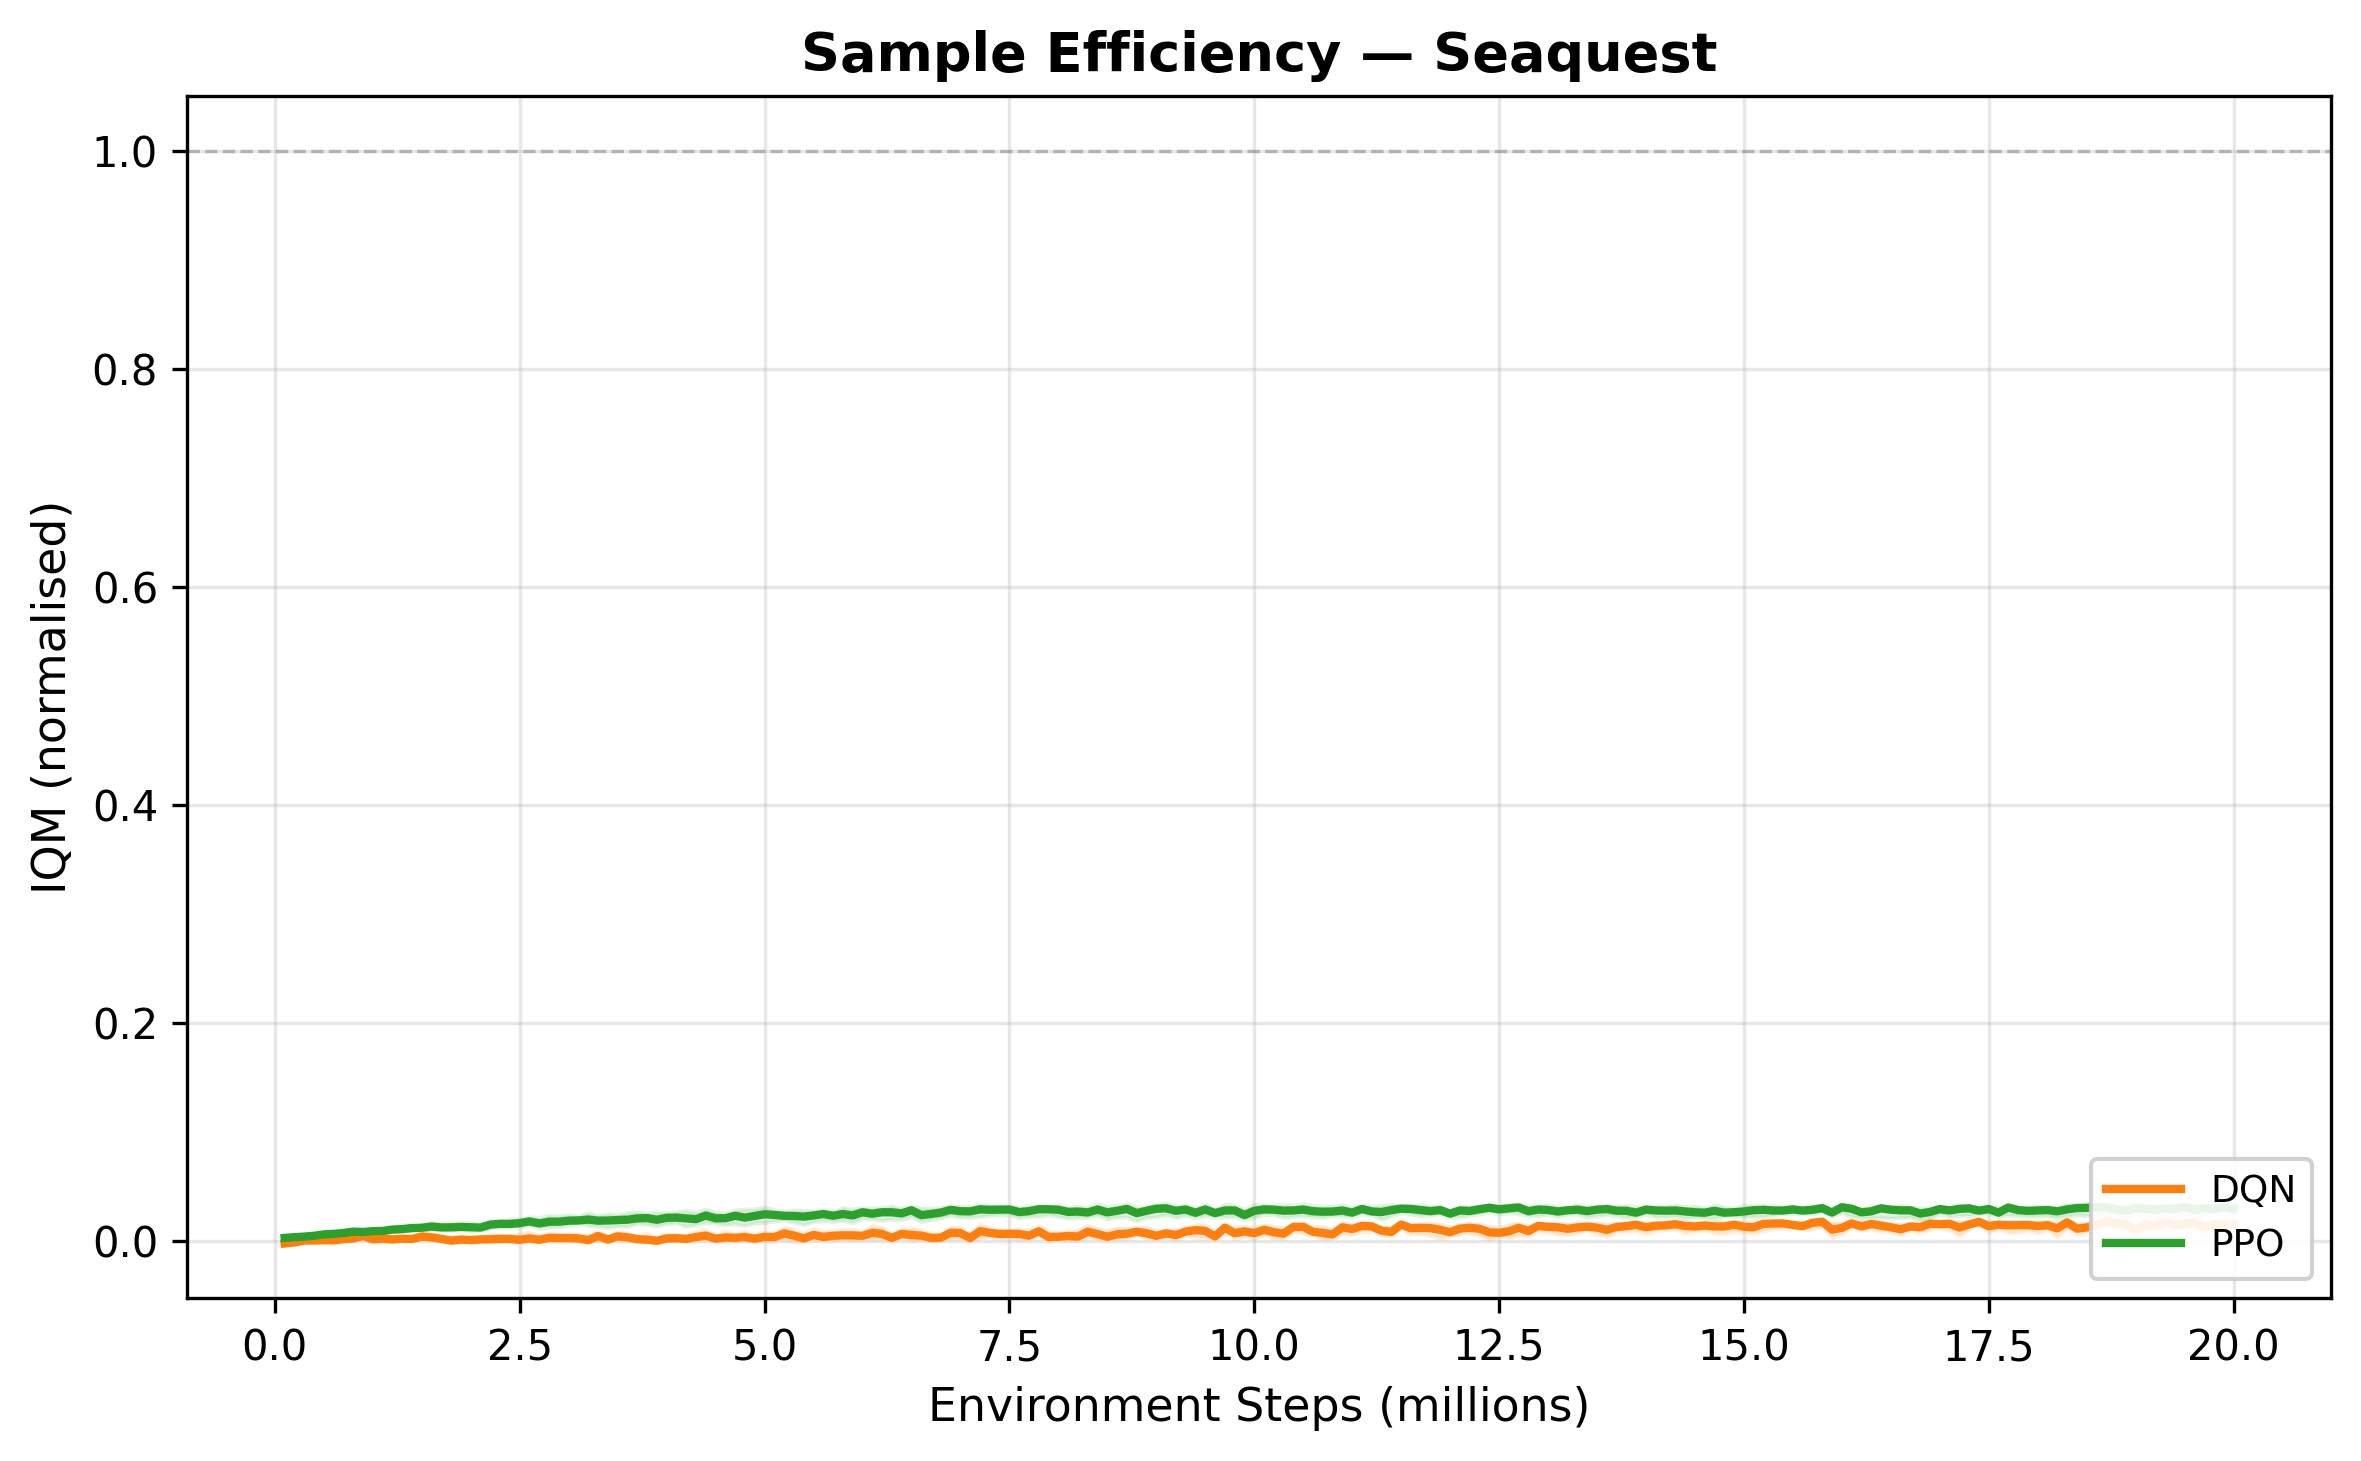
\includegraphics[width=\linewidth]{6_exp3_atari_extended/assets/sample_efficiency_seaquest.png}
    \caption{Seaquest}
  \end{subfigure}
  \caption{Sample efficiency (normalised AUC) per environment at the 20M-step budget.}
  \label{fig:exp3-sample-eff}
\end{figure}

%% ------------------------------------------------------------------
\section{Reproducibility Finding}
\label{sec:exp3-reproducibility}

Beyond the algorithm comparison, Experiment~3 yielded a useful secondary result: the training pipeline is \emph{bitwise deterministic} on the target hardware. Retrained seeds produce identical final evaluation scores and identical checkpoint-by-checkpoint learning curves when run on the same RTX~4090 with the same seeding setup and \texttt{torch.use\_deterministic\_algorithms(True)}. This is unusual for GPU-based RL --- the default assumption in the literature \citep{henderson2018matters} is that GPU non-determinism makes exact bitwise reproduction infeasible.

\begin{figure}[htbp!]
  \centering
  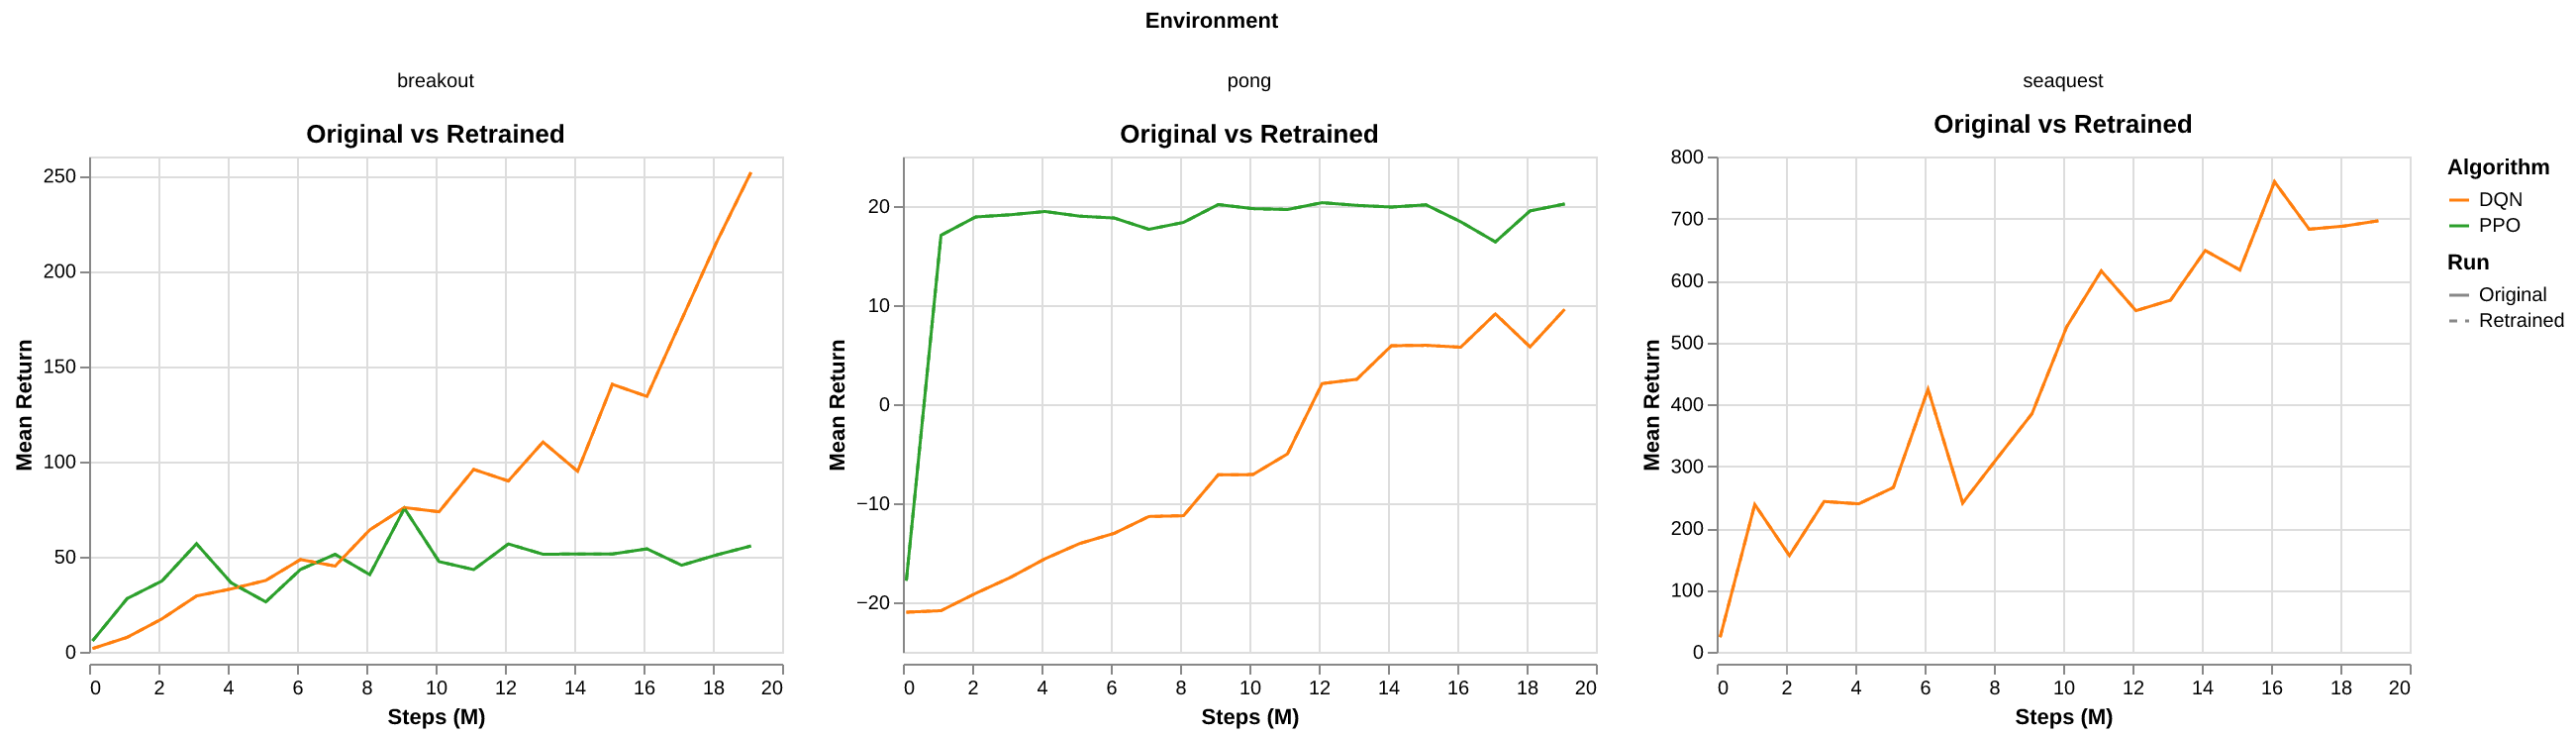
\includegraphics[width=\linewidth]{6_exp3_atari_extended/assets/reproducibility_learning_curves.png}
  \caption[Reproducibility: original vs retrained learning curves]{Original vs retrained learning curves. The two runs of each seed are
           indistinguishable within floating-point noise.}
  \label{fig:exp3-repro-lc}
\end{figure}

\begin{figure}[htbp!]
  \centering
  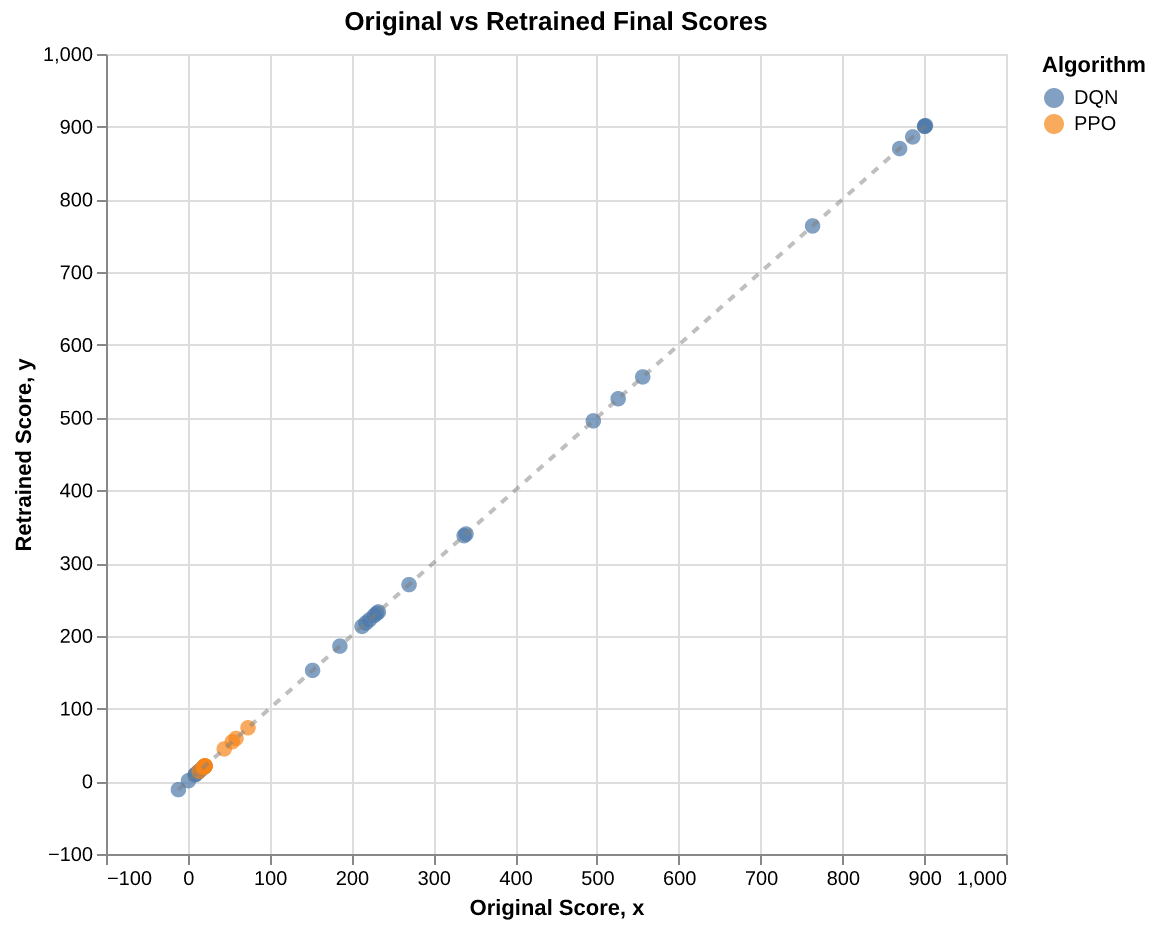
\includegraphics[width=0.65\linewidth]{6_exp3_atari_extended/assets/reproducibility_scatter.png}
  \caption[Reproducibility: original vs retrained final scores]{Original vs retrained final scores. Perfect diagonal agreement
           ($r^2 \approx 1.0$; residuals at the floating-point noise floor).}
  \label{fig:exp3-repro-scatter}
\end{figure}

Future students attempting to reproduce this thesis on an RTX~4090 with the pinned PyTorch and CUDA versions should expect exact numerical agreement with the results reported here.

%% ------------------------------------------------------------------
\section{Timing Analysis}
\label{sec:exp3-timing}

\begin{figure}[htbp!]
  \centering
  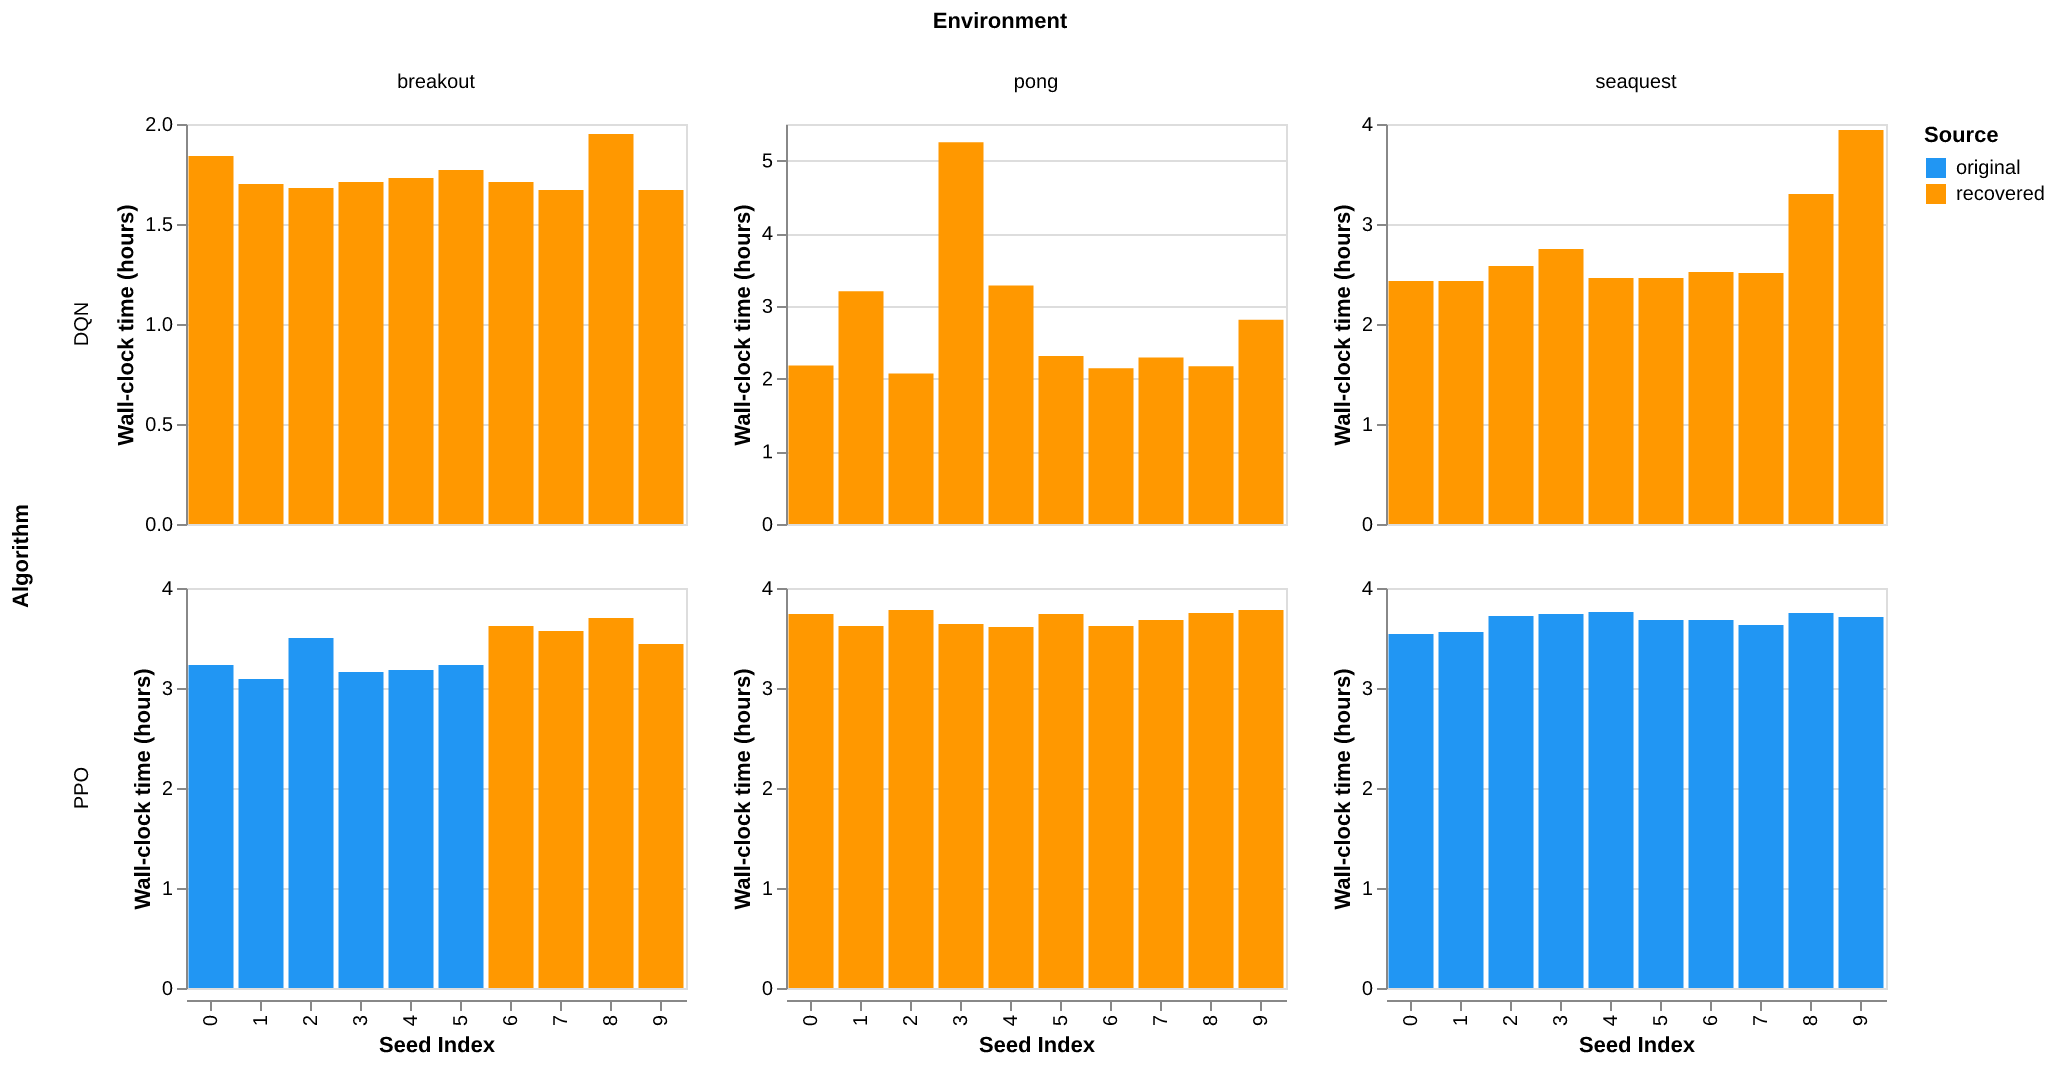
\includegraphics[width=\linewidth]{6_exp3_atari_extended/assets/timing_per_seed.png}
  \caption[Per-seed wall-clock training time: Pong, Breakout, Seaquest]{Per-seed wall-clock training time (hours) for all 60 seeds.
           Timing is complete for both algorithms across all three environments.}
  \label{fig:exp3-timing}
\end{figure}

Table~\ref{tab:exp3-timing} summarises the total wall-clock training time per
algorithm and environment. DQN trained consistently faster than PPO across all
three environments: DQN per-seed averages range from 1.7\,h (Breakout) to 2.8\,h
(Pong), while PPO averages 3.2--3.7\,h per seed. This is somewhat counterintuitive
--- DQN maintains a large replay buffer and performs off-policy gradient updates,
whereas PPO's on-policy rollout collection runs across 16 parallel environments ---
but PPO's rollout collection is more CPU-bound and its update phase runs multiple
epochs of minibatch SGD per rollout, making it heavier per wall-clock step.

DQN Breakout was the fastest cell in the entire experiment at $\approx$1.7\,h/seed,
reflecting that Breakout episodes end quickly once the ball falls through. Seaquest
is the slowest for PPO ($\approx$3.7\,h/seed) due to longer, more complex episodes.

\begin{table}[htbp!]
\centering
\caption{Wall-clock training time per algorithm and environment (20M steps/seed).}
\label{tab:exp3-timing}
\begin{tabular}{llccc}
\toprule
\textbf{Algo} & \textbf{Env} & \textbf{Seeds} & \textbf{Total (h)} & \textbf{Avg/seed (h)} \\
\midrule
DQN & Pong     & 10/10 & 27.7 & 2.8 \\
DQN & Breakout & 10/10 & 17.4 & 1.7 \\
DQN & Seaquest & 10/10 & 27.4 & 2.7 \\
PPO & Pong     & 10/10 & 37.0 & 3.7 \\
PPO & Breakout & 10/10 & 33.7 & 3.4 \\
PPO & Seaquest & 10/10 & 36.8 & 3.7 \\
\midrule
\multicolumn{2}{l}{DQN total} & 30/30 & 72.5 & --- \\
\multicolumn{2}{l}{PPO total} & 30/30 & 107.5 & --- \\
\bottomrule
\end{tabular}
\vspace{0.5em}

\noindent{\small Timing recovered via deterministic retraining (same code, seeds, and hardware).}
\end{table}

%% ------------------------------------------------------------------
\section{Key Findings: Expectations vs Reality}
\label{sec:exp3-key-findings}

\begin{itemize}
  \item \textbf{H3.1 (PPO wins Pong) --- confirmed.} PPO mean 19.78 vs DQN 11.20.
  \item \textbf{H3.2 (DQN wins Breakout) --- confirmed, and larger than expected.} DQN 229 vs PPO 65, a $3.5\times$ margin.
  \item \textbf{H3.3 (both make progress on Seaquest) --- confirmed.} DQN 714, PPO 1174. Both clearly above the random baseline ($\approx68$).
  \item \textbf{H3.4 (Exp~2 aggregate survives) --- \emph{partially refuted}.} The IQM aggregate now favours DQN; the pairwise POI still favours PPO. This is the chapter's central finding.
  \item \textbf{H3.5 (aggregates fragile at $M=3$) --- confirmed.} The IQM/POI disagreement is direct evidence that $M=3$ is still too small for cross-env aggregates to be robust to the choice of summary statistic.
\end{itemize}

%% ------------------------------------------------------------------
\section{Discussion}
\label{sec:exp3-discussion}

\paragraph{Why does the aggregate flip?}
In Experiment~2 (Pong + Breakout, 5M steps), PPO's Pong dominance was large enough to carry the cross-env aggregate despite DQN's Breakout advantage. In Experiment~3, two things change. First, DQN's Breakout lead grows: with $4\times$ more training steps, DQN's value-based learning gets to exploit more of Breakout's state space, pushing the DQN/PPO Breakout ratio from roughly $1.3$ to $3.5$. Second, adding Seaquest introduces a third environment where the gap is moderate, diluting Pong's influence on the aggregate. The net effect is that DQN's Breakout tail drives the IQM up, while PPO's consistent per-seed advantage on Pong and Seaquest means it wins more pairwise comparisons.

\paragraph{The aggregation contradiction.}
IQM is robust to outliers by trimming the top and bottom 25\% of pooled scores; pairwise POI is computed per seed per environment without trimming and then averaged. Breakout is responsible for the flip: DQN's extreme Breakout dominance lifts its IQM through the upper tail, while PPO's consistent advantage on two out of three environments lets it win the majority of pairwise comparisons. Both statistics are valid; they measure different things. I report both rather than choosing one, and treat per-environment results as the primary evidence.

\paragraph{Buffer size oversight.}
The DQN runs used \texttt{buffer\_size=100{,}000} with \texttt{optimize\_memory\_usage=True}. The intended configuration was a 400K buffer (closer to the original Nature DQN paper). All DQN numbers reported here use the 100K buffer. A follow-up study with the intended 400K buffer would quantify how much of DQN's Breakout lead is buffer-size sensitive. I expect the qualitative finding --- DQN wins Breakout, PPO wins Pong and Seaquest --- to survive.

\paragraph{Limitations.}
\begin{itemize}
  \item \textbf{Default hyperparameters.} No per-algorithm or per-environment tuning. The comparison is between out-of-the-box SB3 DQN and PPO at the 20M-step budget.
  \item \textbf{Seed count.} 10 seeds per cell, matching Experiment~2 but fewer than Experiment~1's 15. Bootstrap CIs are correspondingly wider.
  \item \textbf{$M=3$ environments.} Still small. The IQM/POI disagreement is direct evidence that $M=3$ is insufficient for robust cross-env aggregates.
  \item \textbf{DQN buffer size.} 100K instead of the intended 400K (oversight during training-script configuration).
  \item \textbf{Training timing.} Original wall-clock logs were lost. Retrained runs recovered full DQN timing; PPO timing is partially incomplete. Evaluation scores are complete for all 30 runs.
\end{itemize}
